\documentclass[a4j]{ujarticle}
\usepackage[dvipdfmx]{graphicx}
\usepackage{url}
\usepackage{bbding}
\usepackage{lscape}
\usepackage[subrefformat=parens]{subcaption}
\usepackage{bm}
\usepackage{amsmath}
\usepackage{ascmac}
% \usepackage{minipage}

\title{進捗報告資料}
\author{安達智哉\\to-adachi@ist.osaka-u.ac.jp}
\date{2019年12月4日}

\begin{document}
\maketitle

% \section{CQ研究会}
% \subsection{質疑応答}
%   \begin{itemize}
%     \item  端末1台1台の通信周期は固定か? 端末の通信周期はアプリケーション毎なのか?\\
%     $\rightarrow$ 本評価では、端末の通信周期は固定である。また、シナリオ2ではアプリケーションごとに通信周期が異なることを想定している。
%     \item default bearerやdedicated bearerなどのベアラがあり、一台の端末が複数のベアラを持つこともできるが、それにも提案手法を適用できるか?\\
%     $\rightarrow$ 現在、複数のベアラを使って通信するようなアプリケーションを想定した提案や評価はできていないため、今後の課題である。一方で、そのような複数ベアラを用いた通信は一般的ではないこともあるため、単一ベアラを対象とした手法でも十分であると言える。
%   \end{itemize}
% \subsection{コメント}
%   \begin{itemize}
%     \item Connected inactive はSYN floodingと同じように、メモリへの攻撃になるのかも。\\
%     $\rightarrow$ Idleタイマをリソース需要に応じて変化させることにより、攻撃に被害を抑制できる可能性がある。Idleタイマの動的制御に関しては、今後の課題である。
%     \item プライベートLTEやローカル5Gなど、一般の企業や個人が自前でモバイルネットワークを構築可能な環境が現在開発されている。これらは、限られたサーバ資源の上で動作する必要があるため、提案手法のような、限られたノード資源を効率的に利用する方法の相性が良いかも。
%     \item MMEが処理できるシグナリング数の限界値は実験に基づいて設定したようだけれど、実際にはCPU負荷は変動が大きいので難しい。
%   \end{itemize}
% - 研究会質疑について
% -- ネットワーク側からは周期はわからない、ということは伝えるべきでしたね。
% -- 各端末は1つのベアラ (default ベアラ) だけを設定する、ということは、
%   説明した方がいいですね。提案方式もそれが前提となっているし、評価の
%   設定も。
%
% - DoS攻撃軽減について
% -- いったんアクティブになった端末のタイマは変更できない、という場合に
%   は、防止は難しいですね。(Inactiveになってそのまま黙られると、メモリ
%   使われてしまう) 後続で接続してくる端末に対しては対応できるけど。
% - CPU変動が激しいのは負荷が高い時のようなので、CPU負荷の監視をどうする
%  か、ですね。なので、一般的なサーバのCPU負荷の監視、という話で、探せ
%  ば、方式はあると思う。


%
% \section{Idleタイマの制御方法}
% \label{sec:hard-state}
% 本節では、UEの強制的な状態変化を引き起こさないことを前提にする。
% つまり、Idleタイマが切れていないUEを強制的にIdle状態へ遷移させることはないとする。
% また、Idleタイマの更新は、UEがデータ送信を行うタイミングで実行するものとする。
% MMEはUEを収容するために使用されているCPUおよびメモリリソース量を観測できるものとする。
% つまり、UEの収容とは無関係な処理によって発生する負荷を取り除いたCPU負荷およびメモリ使用量を知ることができるとする。
% MMEは現在収容されているUE台数を観測できるものとする。
%
% 突発的な負荷の増加に対応するという観点から、現在収容しているUEに加え、最も多くのUEを収容できるようなIdleタイマの値が最適と考える。
% 具体的には、現在収容しているUEと同じ通信周期を持つUEがネットワークに参加すると仮定し、収容可能なUE台数が最大となるIdleタイマの値を最適と定義する。
% また、CPUよびメモリのどちらも過負荷状態でないことは、UEを収容可能であることの必要十分条件であるとする。
%
% まず、UE一台あたりが各リソースに与える負荷の平均を推定する。
% 現在収容しているUE台数を$N_{\rm UE}$とする。
% UE台数が$N_{\rm UE}$、Idleタイマが$T$の時に観測される、CPU負荷およびメモリ使用量をそれぞれ$C_{N_{\rm UE}}(T)$、$M_{N_{\rm UE}}(T)$とする。
% この時、UE一台あたりが与えるCPU負荷およびメモリ使用量の平均($C_{1}(T)$、$M_{1}(T)$)は以下の式(\ref{eq:cpu_1})、(\ref{eq:memory_1})で表せる。
% \begin{eqnarray}
%    C_{1}(T) =& \frac{C_{N_{\rm UE}}(T)}{N_{\rm UE}}\label{eq:cpu_1}\\
%    M_{1}(T) =& \frac{M_{N_{\rm UE}}(T)}{N_{\rm UE}}\label{eq:memory_1}
% \end{eqnarray}
%
% Idleタイマを$T$とした時に、収容可能なUEの総数を$N_{\rm UE}^{\rm capa}(T)$とする。
% $N_{\rm UE}^{\rm capa}(T)$は、$C_{1}(T)$、$M_{1}(T)$、$C^{\rm max}$および$M^{\rm max}$を用いて、以下の式(\ref{eq:UE_add})で表せる。
% ここで、$C^{\rm max}$、$M^{\rm max}$はそれぞれシグナリング処理およびUEのセッション情報を保持するために使用可能なCPUリソース量およびメモリリソース量である。
% \begin{eqnarray}
%    N_{\rm UE}^{\rm capa}(T) =& \lfloor  \min \{\frac{C^{\rm max}}{C_{1}(T)},\frac{M^{\rm max}}{M_{1}(T)}\} \rfloor \nonumber\\
%    =& \lfloor N_{\rm UE} \cdot \min \{\frac{C^{\rm max}}{C_{N_{\rm UE}}(T)}, \frac{M^{\rm max}}{M_{N_{\rm UE}}(T)}\} \rfloor\label{eq:UE_add}
% \end{eqnarray}
% Idleタイマを制御する上での目的関数を以下の式(\ref{eq:objective_function})に示す。
% \begin{eqnarray}
%   \text{maximize} :& N_{\rm UE}^{\rm capa}(T)
%   \label{eq:objective_function}
% \end{eqnarray}
%
%
%
% $N_{\rm UE}^{\rm capa}(T)$を最大化するIdleタイマの値が明らかである場合は、その値をIdleタイマに設定すれば良い。
% しかし一般的に、UEの台数や通信周期は未知であり時間的に変動するため、$N_{\rm UE}^{\rm capa}(T)$を最大化するIdleタイマの値を知ることは難しい。
% そのような場合は、$N_{\rm UE}^{\rm capa}(T)$を最大化するように、Idleタイマを適応的に制御する必要がある。
% 具体的には、各リソースの使用量を観測して、$N_{\rm UE}^{\rm capa}(T)$を大きくする向きにIdleタイマを変化させる。
% このステップを複数回繰り返すことにより、Idleタイマを制御する。
%
% この時、1ステップごとのIdleタイマの変化量を考える必要がある。
% この値を小さく設定すると、最適な値に到達するまでに大きな時間がかかってしまう場合がある。
% 逆にIdleタイマの変化量を大きく設定すると、Idleタイマが発振する可能性もあり、制御が不安定になる。
% また、UEの通信周期によって、Idleタイマが変化した時に各リソースの負荷の変化量が異なる点も考慮する必要がある。
% つまり、ネットワークの変化に短い時間スケールで対応しつつ、安定した制御を実現するためには、ネットワークの環境に応じてIdleタイマの変化量を制御する仕組みが必要である。
% このような制御には様々な手法が考えられるが、本報告では動作がシンプルであり、汎用性が高いPID制御を用いる。
% $T$および$N_{\rm UE}^{\rm capa}(T)$をそれぞれ、PID制御における入力値および出力値として捉えることで、Idleタイマの変化量を調整しつつ、最適値に近づけることができる。
%
% まず、PID制御における出力値$y(t)$および目標値$r(t)$を設定する。
% 以前の評価より、UE台数を固定した時、CPU負荷はIdleタイマの値に対して広義単調減少でありかつ、メモリ使用量はIdleタイマの値に対して広義単調増加であることがわかっている。
% このことから、式(\ref{eq:UE_add})を確認すると、$\frac{C^{\rm max}}{C_{N_{\rm UE}}(T)}$は広義単調増加でありかつ、$\frac{M^{\rm max}}{M_{N_{\rm UE}}(T)}$は広義単調減少であることがわかる。
% ここで、$\frac{C^{\rm max}}{C_{N_{\rm UE}}(T)}$と$\frac{M^{\rm max}}{M_{N_{\rm UE}}(T)}$の差分を最小化するような$T$の集合を$\bm{T}$とする。また、$N_{\rm UE}^{\rm capa}(T)$を最大化するような$T$の集合を$\bm{T}_{\rm optimal}$とする。すると、$T\in\bm{T}$であることは$T\in\bm{T}_{\rm optimal}$であるための十分条件になる。
%
% 以上の議論のイメージを図\ref{theory_1_all_30s_theory}、図\ref{theory_1_add_C_M}および図\ref{theory_1_add_all}に示す。
% 図\ref{theory_1_all_30s_theory}はUE台数が500,000台,UEごとの通信周期は10~sから6,000~sの範囲で一様分布とした時の、Idleタイマと各リソース負荷の関係を示したものである。
% 図\ref{theory_1_add_C_M}は図\ref{theory_1_all_30s_theory}と同じUEを収容した時の、Idleタイマと$N_{\rm UE} \cdot \frac{C^{\rm max}}{C_{N_{\rm UE}}(T)}$と$N_{\rm UE} \cdot \frac{M^{\rm max}}{M_{N_{\rm UE}}(T)}$との関係を示している。
% また、図\ref{theory_1_add_all}は図\ref{theory_1_all_30s_theory}と同じUEを収容した時の、Idleタイマと$N_{\rm UE}^{\rm capa}(T)$との関係を示している。
% 図\ref{theory_1_add_all}を見ると、$N_{\rm UE}^{\rm capa}(T)$を最大化するIdleタイマの値と$\frac{C^{\rm max}}{C_{N_{\rm UE}}(T)}$と$\frac{M^{\rm max}}{M_{N_{\rm UE}}(T)}$の差分を最小化するIdleタイマの値が一致していることが確認できる。
%
% \begin{figure}[htbp]
%   \begin{center}
%     \begin{tabular}{c}
%       \begin{minipage}{1\hsize}
%         \begin{center}
%           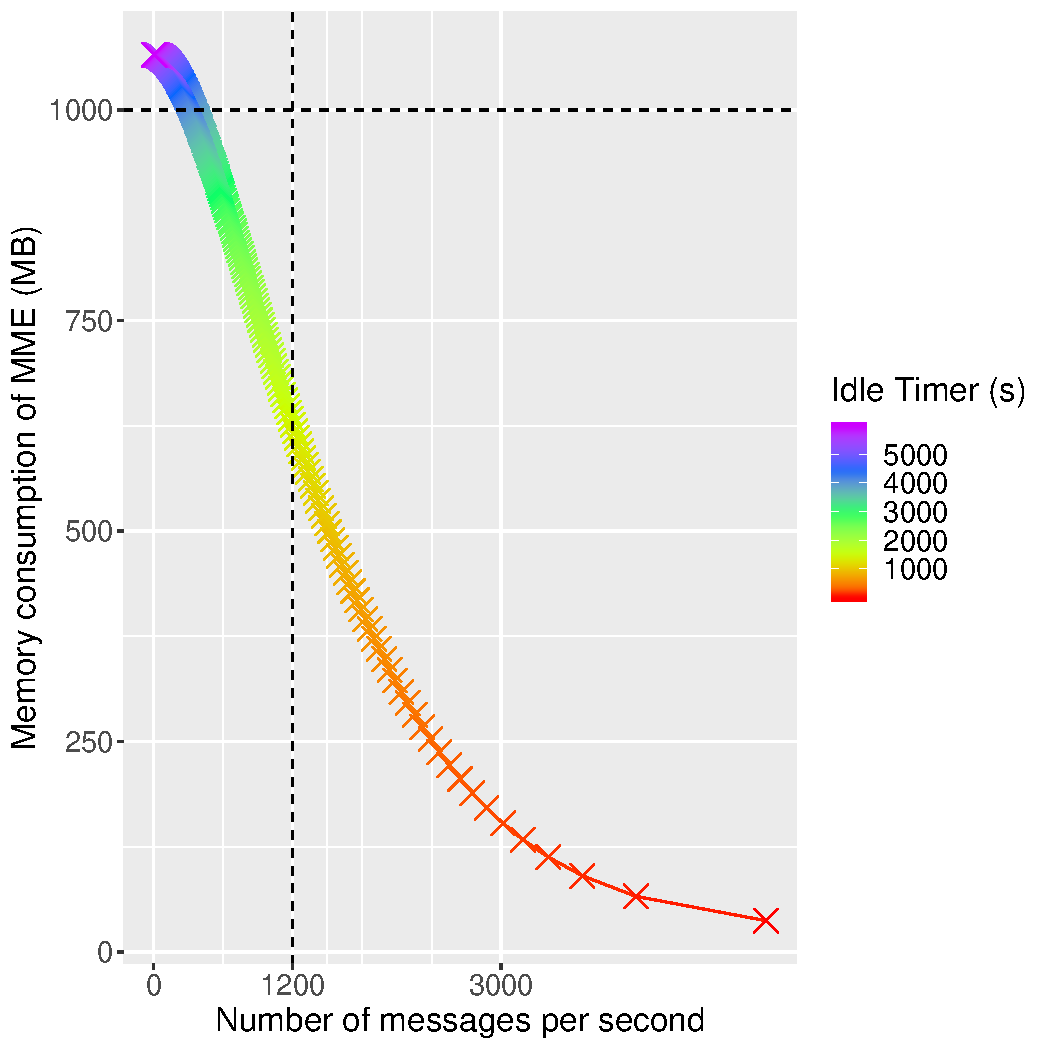
\includegraphics[width=0.6\hsize]{theory_1_all_30s_theory.pdf}
%           \caption{Idleタイマに対する,メッセージ処理頻度とメモリ使用量の関係}
%           \label{theory_1_all_30s_theory}
%         \end{center}
%       \end{minipage}
%     \end{tabular}
%   \end{center}
% \end{figure}
%
% \begin{figure}[htbp]
%   \begin{center}
%     \begin{tabular}{c}
%       \begin{minipage}{0.47\hsize}
%         \begin{center}
%         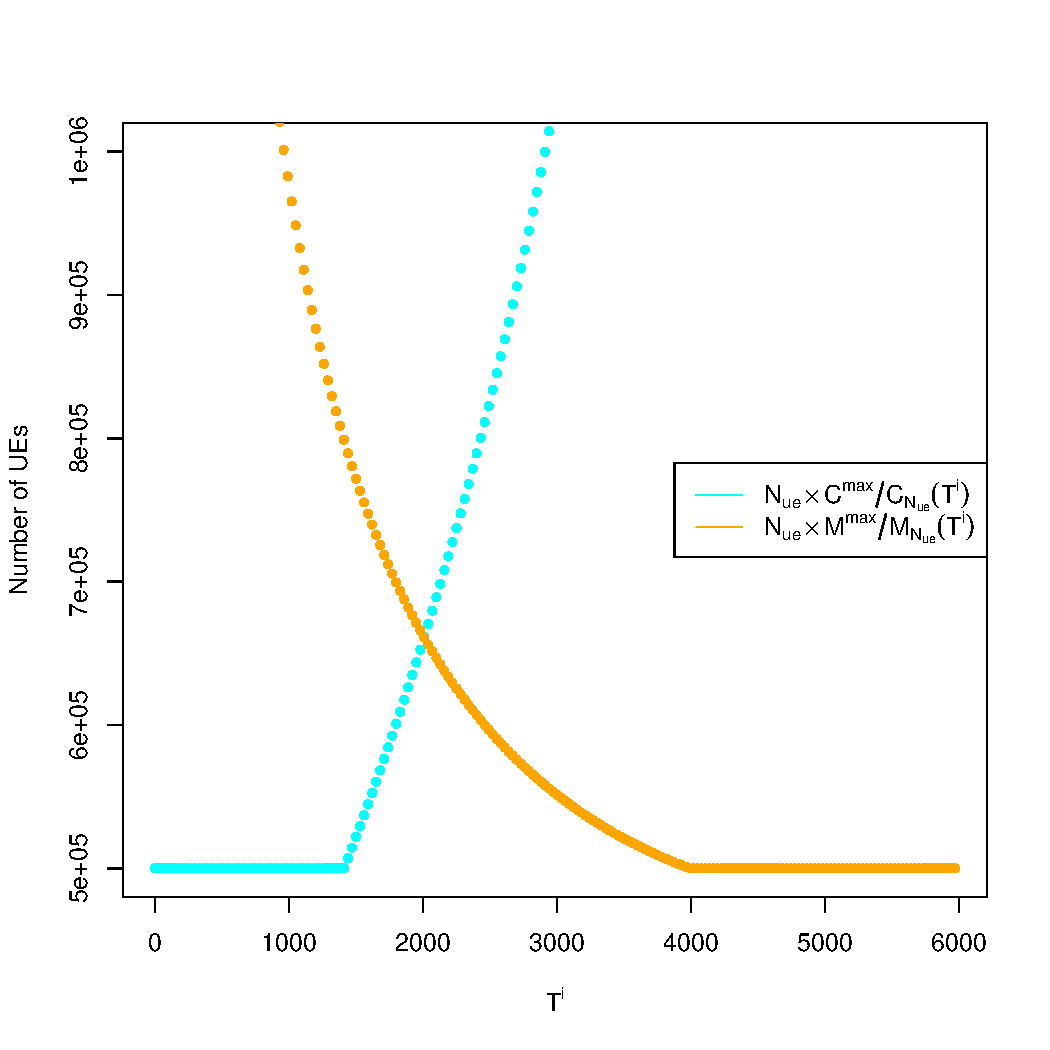
\includegraphics[width=1\hsize]{theory_1_add_C_M.pdf}
%         \subcaption{Idleタイマと$N_{\rm UE} \cdot \frac{C^{\rm max}}{C_{N_{\rm UE}}(T)}$と$N_{\rm UE} \cdot \frac{M^{\rm max}}{M_{N_{\rm UE}}(T)}$の関係}
%         \label{theory_1_add_C_M}
%         \end{center}
%       \end{minipage}
%       \begin{minipage}{0.47\hsize}
%         \begin{center}
%         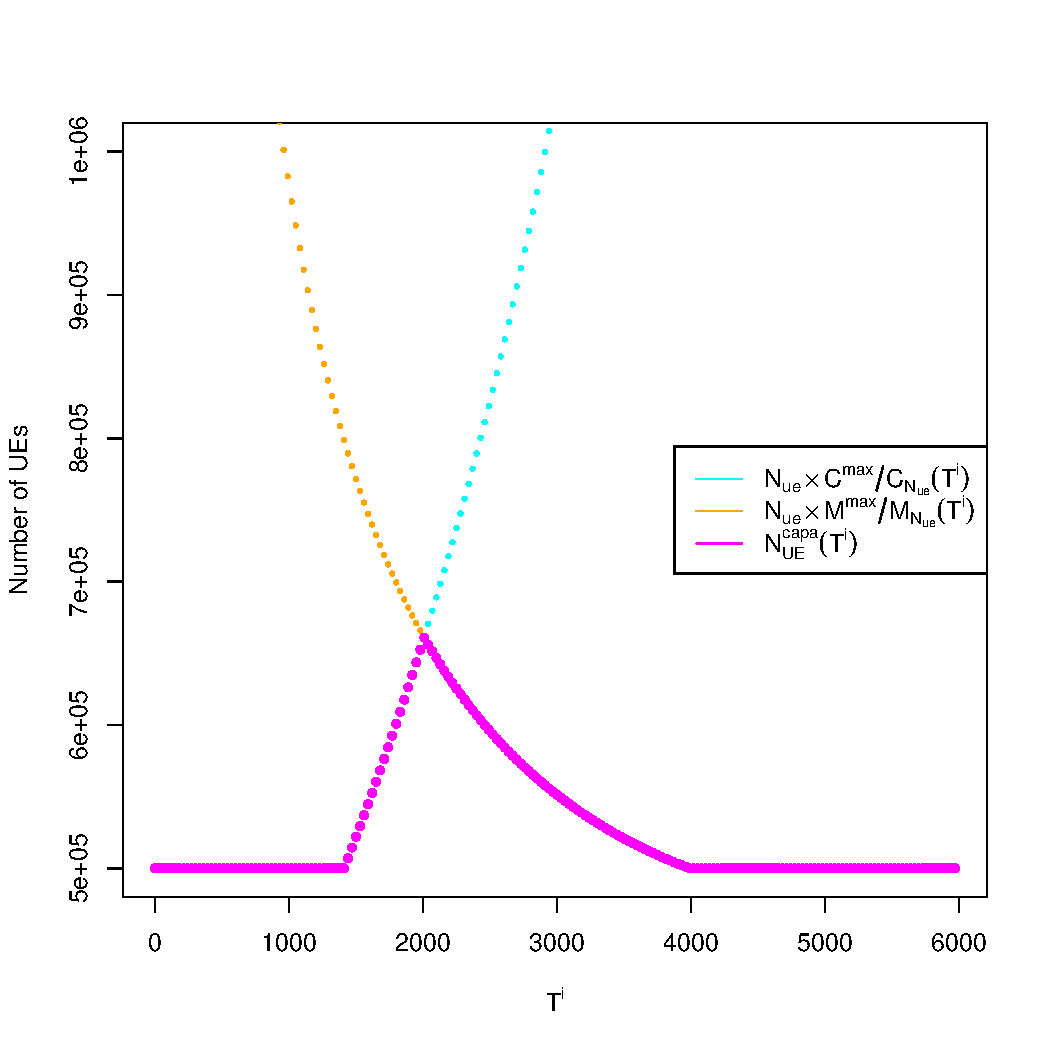
\includegraphics[width=1\hsize]{theory_1_add_all.pdf}
%         \subcaption{Idleタイマと$N_{\rm UE}^{\rm capa}(T)$の関係}
%         \label{theory_1_add_all}
%         \end{center}
%       \end{minipage}
%     \end{tabular}
%     \caption{}
%   \end{center}
% \end{figure}
%
% このことを踏まえ、PID制御における出力値$y(t)$および目標値$r(t)$を以下の式(\ref{eq:PID_y_t})、(\ref{eq:PID_r_t})のように定義する。
% $t$は時刻を表す変数である。
% \begin{eqnarray}
%   y(t) &=& \frac{C^{\rm max}}{C_{N_{\rm UE}}(T)} - \frac{M^{\rm max}}{M_{N_{\rm UE}}(T)}
%   \label{eq:PID_y_t} \\
%   r(t) &=& 0
%   \label{eq:PID_r_t}
% \end{eqnarray}
%
%
% 時刻$t$における$y(t)$と$r(t)$の差を$e(t)$として以下の式(\ref{eq:PID_e_t})ように定義すると、PID制御における操作量($u(t)$)は以下の式(\ref{eq:PID_u_t})で表せる。
% \begin{eqnarray}
%   e(t) &=& r(t) - y(t)
%   \label{eq:PID_e_t} \\
%   u(t) &=& K_p \cdot e(t) + K_i \cdot \int_0^t e(\tau) d\tau + K_d \cdot \frac{de(t)}{dt}
%   \label{eq:PID_u_t}
% \end{eqnarray}
% ここで、$K_p$、$K_i$および$K_d$はそれそれ、比例ゲイン、積分ゲインおよび微分ゲインと呼ばれる定数である。
% これらの定数は、$e(t)$およびその積分値、微分値が$u(t)$にどの程度寄与するのかを決定する。

\section{ジーグラニコルスの限界感度法}
\label{gigura}
PID制御においては、比例ゲイン($K_p$)、積分ゲイン($K_i$)、微分ゲイン($K_d$)と呼ばれる3つの定数を設定する必要がある。これらの定数を``ジーグラ・ニコルスの限界感度法"と呼ばれる手順に基づき設定した。

ジーグラ・ニコルスの限界感度法に基づくゲインの求め方を以下に示す。
\begin{description}
  \item[ステップ~1] 積分ゲイン($K_i$)および微分ゲイン($K_d$)を0にして調節器が比例動作だけを行うようにする。
  \item[ステップ~2] 比例ゲイン($K_p$)を0から徐々に大きくしていき、制御量が安定限界に達して一定振幅振動を持続するようになった時に$K_p$の増加を止める。
  \item[ステップ~3] ステップ~2の時の比例ゲインを限界感度($K_u$)、振動周期を限界周期($P_u$)とし、これらの値から各ゲインを以下の表\ref{table:Ziegler-Nichols}のように求める。
  \item[ステップ~4]必要に応じてステップ~3で求めた各ゲインの値を調整する。
\end{description}
\begin{table}[]
  \centering
  \caption{ジーグラ・ニコルスの限界感度法}
  \label{table:Ziegler-Nichols}
  \begin{tabular}{c|c|c|c|c|c}
    \hline
    制御の種類  & $K_p$ & $K_i$ & $K_d$ & $T_i$ & $T_d$ \\\hline \hline
    P & 0.5$K_u$ & 0 & 0 & - & - \\
    PI & 0.45$K_u$ & $K_p/0.83P_u$ & 0 & $0.83P_u$ & - \\
    PID & 0.6$K_u$ & $K_p/0.5P_u$  & $K_p \cdot 0.125P_u$ & $0.5P_u$ & $0.125P_u$ \\\hline
  \end{tabular}
\end{table}

以下のシナリオにおいて、ジーグラニコルスの限界感度法を用いて、PID制御のゲインを求めた。
UE台数は648,000台であり、UEの持つ通信周期は1~day,2~hours,1~hour,30~minutesのいずれかである。それぞれの通信周期を持つUEの割合は表\ref{table:interval}の通りである。また、各パラメータを表\ref{table:parameter}に示す。
\begin{table}[htbp]
  \centering
  \caption{パラメータ設定}
  \label{table:parameter}
  \begin{tabular}{c|l}
    \hline
    Parameter  & Numerical setting \\\hline \hline
    $T^{\rm ci}$ & 10~s\\
    $s_{\rm MME}^{\rm c \to \rm c}$ & 0~messages\\
    $s_{\rm MME}^{\rm ci \to \rm ci}$ & 0~messages\\
    $s_{\rm MME}^{\rm c \to \rm ci}$ & 0~messages\\
    $s_{\rm MME}^{\rm ci \to \rm c}$ & 0~messages\\
    $s_{\rm MME}^{\rm ci \to \rm i}$ & 5~messages\\
    $s_{\rm MME}^{\rm i \to \rm c}$ & 5~messages\\
    $m^{\rm c}_{\rm MME}$ & 17878~bits\\
    $m^{\rm ci}_{\rm MME}$ & 17878~bits\\
    $m^{\rm i}_{\rm MME}$ & 408~bits\\
    $C^{\rm max}$ & 1200~messages/s\\
    $M^{\rm max}$ & 1,000~MB\\
    $d_h$ & 1 \\\hline
  \end{tabular}
\end{table}
\begin{table}[htbp]
  \centering
  \caption{UEの通信周期の分布}
  \label{table:interval}
  \begin{tabular}{c|cccc}
    \hline
    &\multicolumn{4}{c}{通信周期} \\
    & 1~day & 2~hours & 1~hour & 30~minutes \\\hline \hline
    UE台数の割合 & 40\% & 40\% & 15\% & 5\% \\\hline
  \end{tabular}
\end{table}


% まず、限界感度および限界周期を求めるために、$K_i$および$K_d$を0にして、$K_p$を0から徐々に大きくしていった。その結果を図\ref{result_1}および図\ref{result_2}に示す。これらの図は$K_p=0.2$、$K_p=0.5$、$K_p=0.52$、$K_p=0.53$の場合の結果を示している。左側の図は、タイムステップごとの$r(y)$(式(\ref{eq:PID_e_t})より)の変化を示している。右図は、タイムステップごとのIdleタイマの変化を示している。これらの図を見ると、$K_p=0.52$以下の場合は制御が収束するが、$K_p=0.53$の場合は制御が収束せず、一定振幅振動していることがわかる。このことから、限界感度($K_u$)を0.53とする。また、限界周期($P_u$)は図\ref{scenario_5_e_86400_345600_053_0_0}より、7450~sとする。

限界感度および限界周期を求めるために、$K_i$および$K_d$を0にして、$K_p$を0から徐々に大きくしていった。その結果、$K_p=0.53$の場合は制御が収束せず、一定振幅振動することがわかった。このことから、限界感度($K_u$)を0.53とする。また、限界周期($P_u$)は図\ref{scenario_5_e_86400_345600_053_0_0}より、7450~sとする。
% \begin{figure}[htbp]
%   \begin{center}
%     \begin{tabular}{c}
%       \begin{minipage}{0.5\hsize}
%         \begin{center}
%         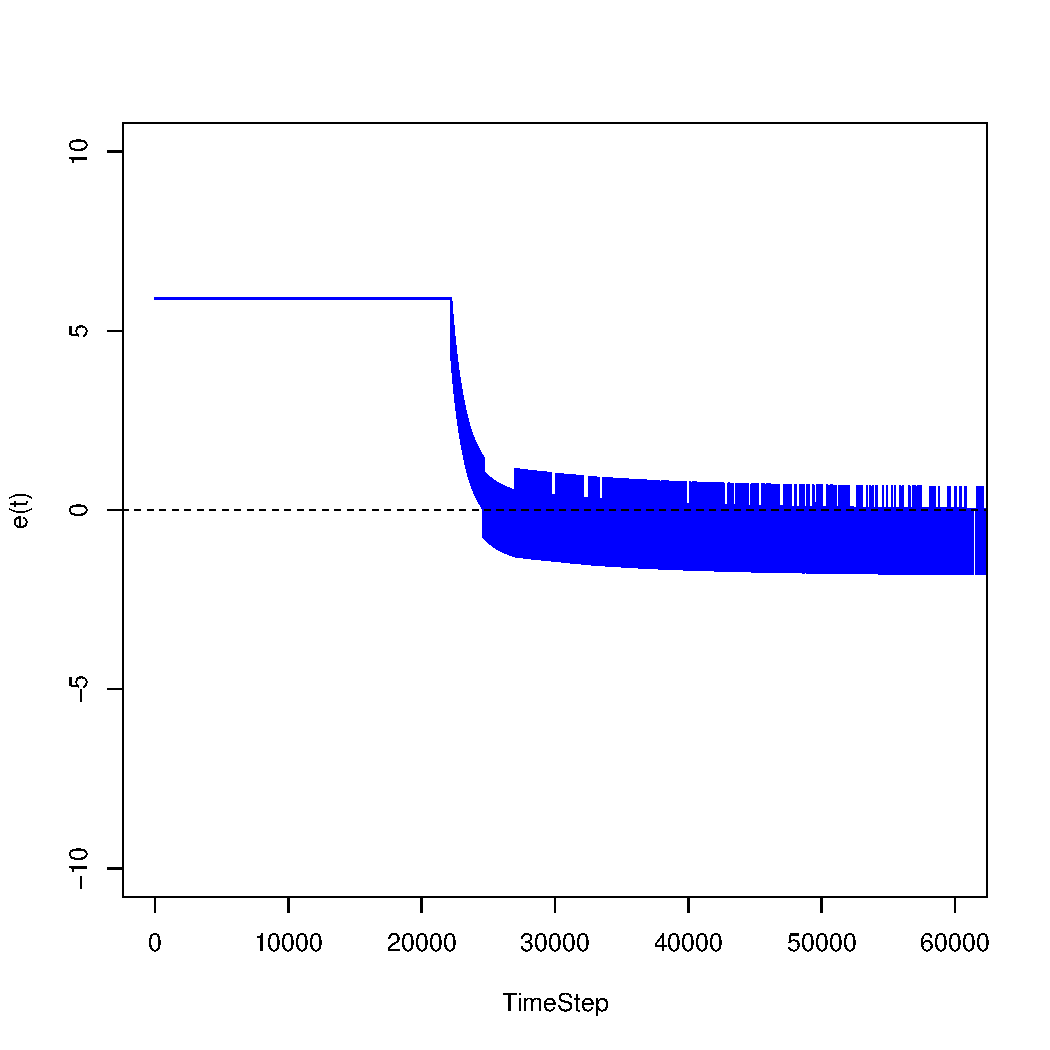
\includegraphics[width=1\hsize]{scenario_5_e_86400_345600_02_0_0.pdf}
%         \subcaption{$e(t)$の変化($K_p = 0.2$)}
%         \label{scenario_5_e_86400_345600_02_0_0}
%         \end{center}
%       \end{minipage}
%       \begin{minipage}{0.5\hsize}
%         \begin{center}
%         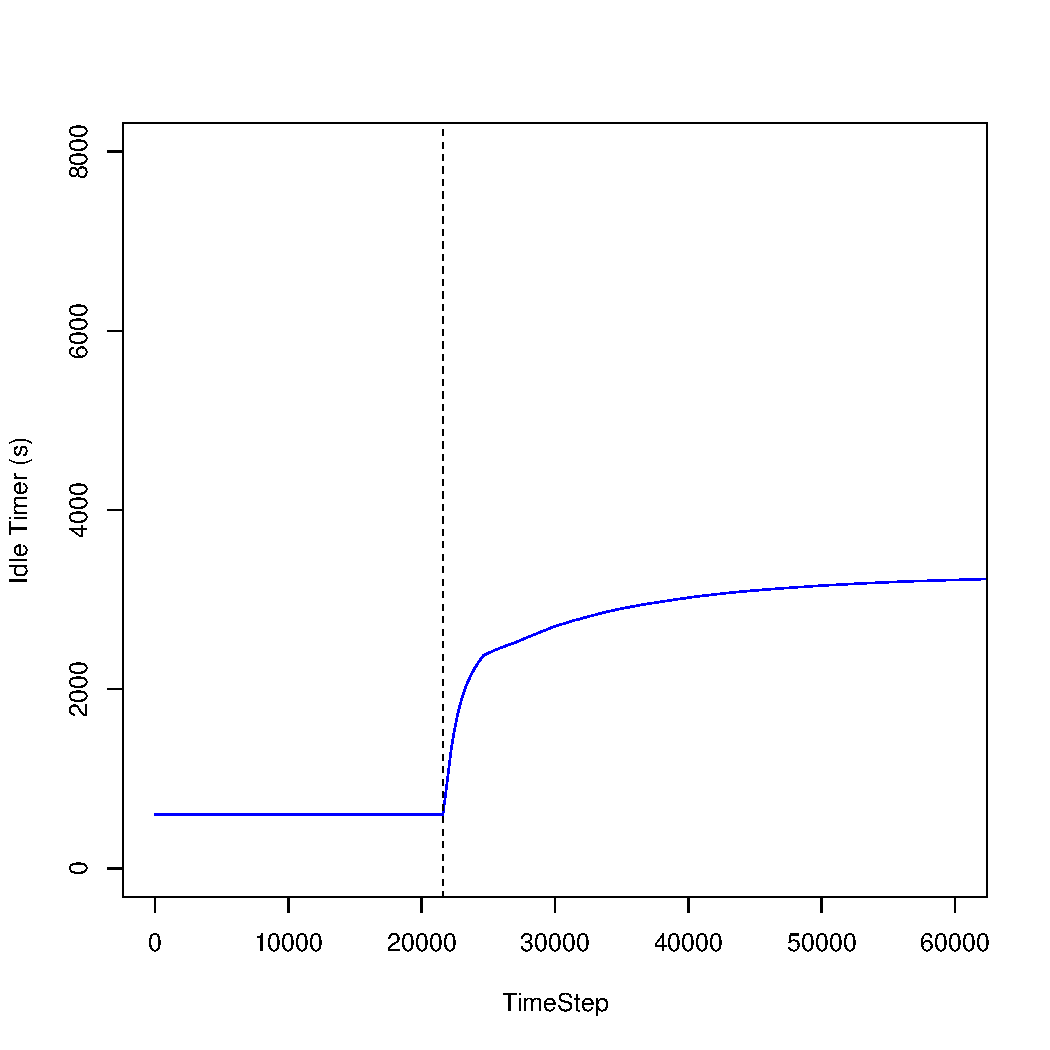
\includegraphics[width=1\hsize]{scenario_5_idleTimer_86400_345600_02_0_0.pdf}
%         \subcaption{IdleTimerの変化($K_p = 0.2$)}
%         \label{scenario_5_idleTimer_86400_345600_02_0_0}
%         \end{center}
%       \end{minipage}\\
%       \begin{minipage}{0.5\hsize}
%         \begin{center}
%         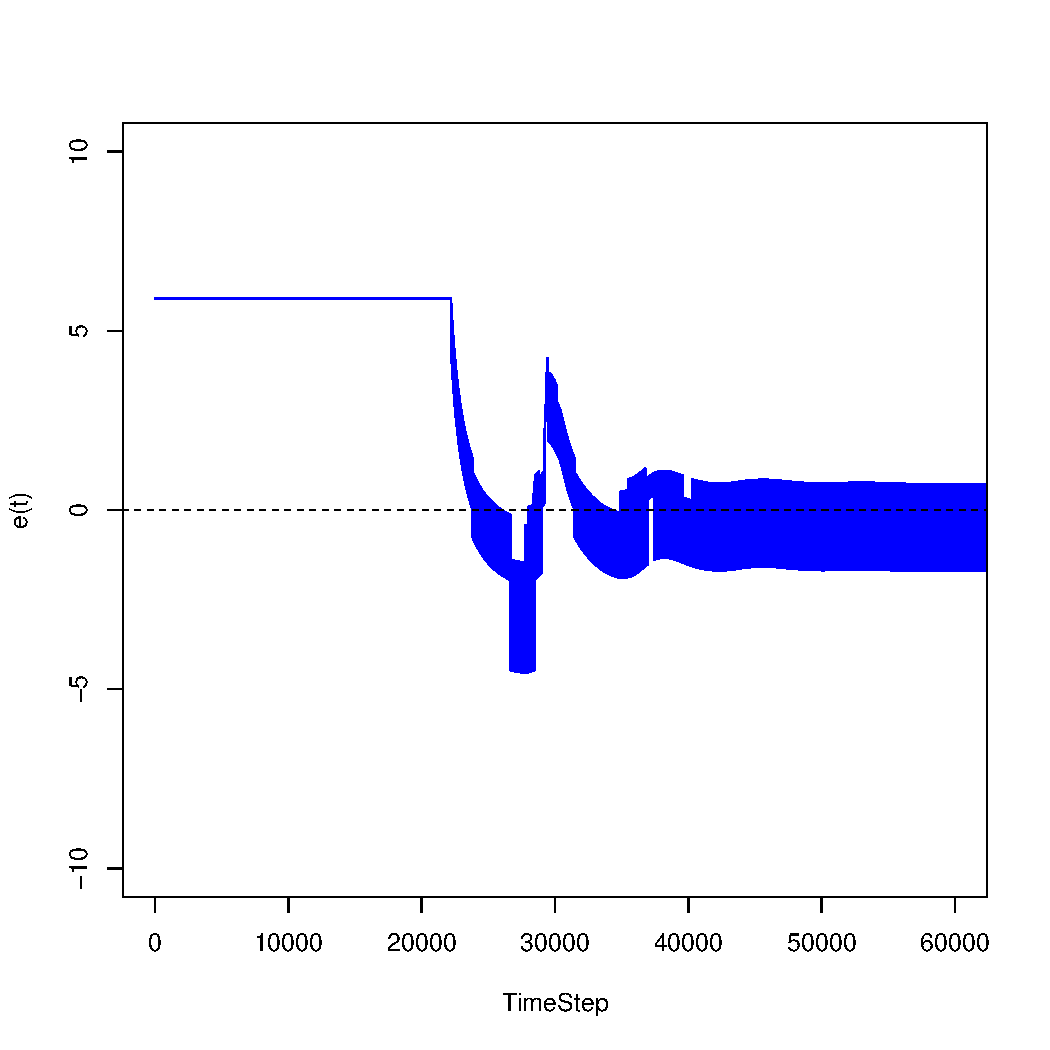
\includegraphics[width=1\hsize]{scenario_5_e_86400_345600_05_0_0.pdf}
%         \subcaption{$e(t)$の変化($K_p = 0.5$)}
%         \label{scenario_5_e_86400_345600_05_0_0}
%         \end{center}
%       \end{minipage}
%       \begin{minipage}{0.5\hsize}
%         \begin{center}
%         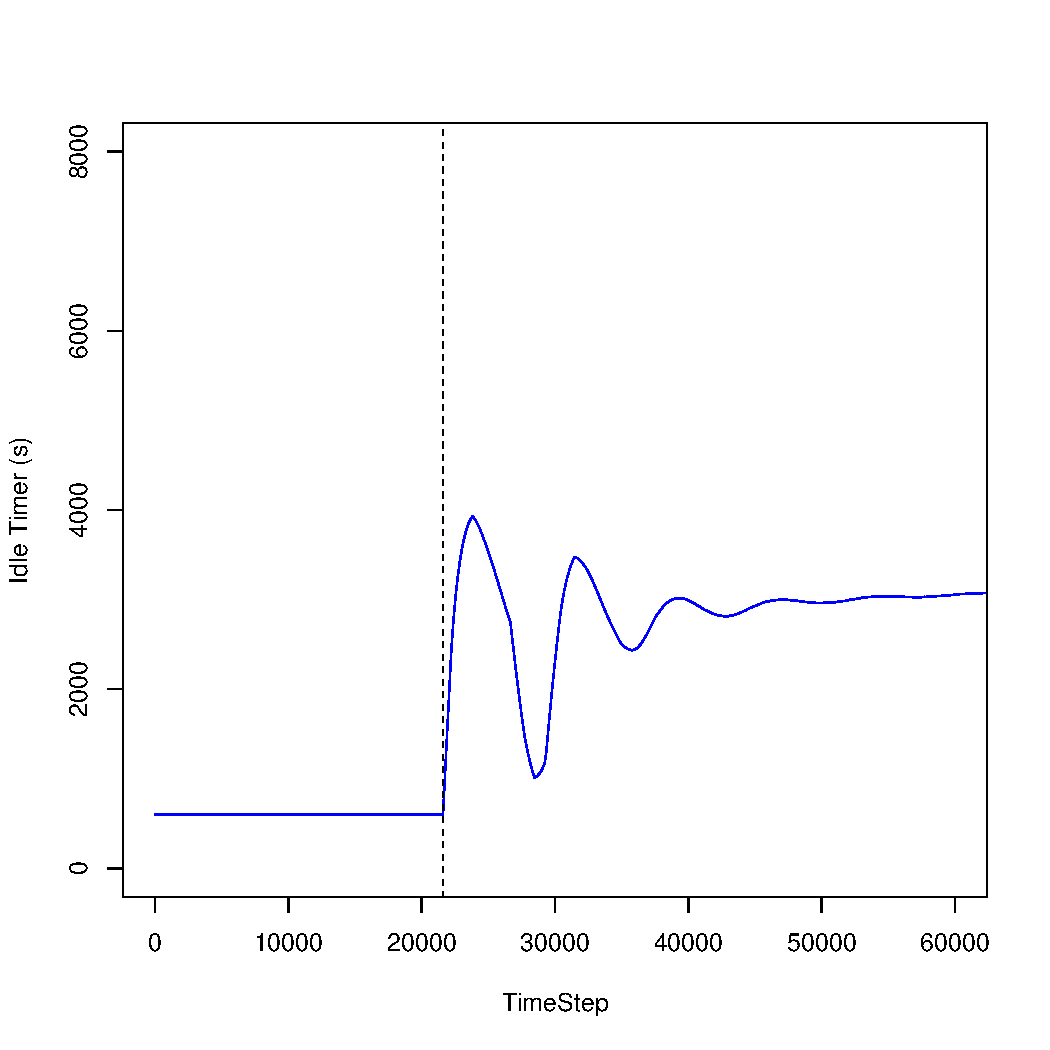
\includegraphics[width=1\hsize]{scenario_5_idleTimer_86400_345600_05_0_0.pdf}
%         \subcaption{IdleTimerの変化($K_p = 0.5$)}
%         \label{scenario_5_idleTimer_86400_345600_05_0_0}
%         \end{center}
%       \end{minipage}
%     \end{tabular}
%     \caption{}
%     \label{result_1}
%   \end{center}
% \end{figure}
% \begin{figure}[htbp]
%   \begin{center}
%     \begin{tabular}{c}
%       \begin{minipage}{0.5\hsize}
%         \begin{center}
%         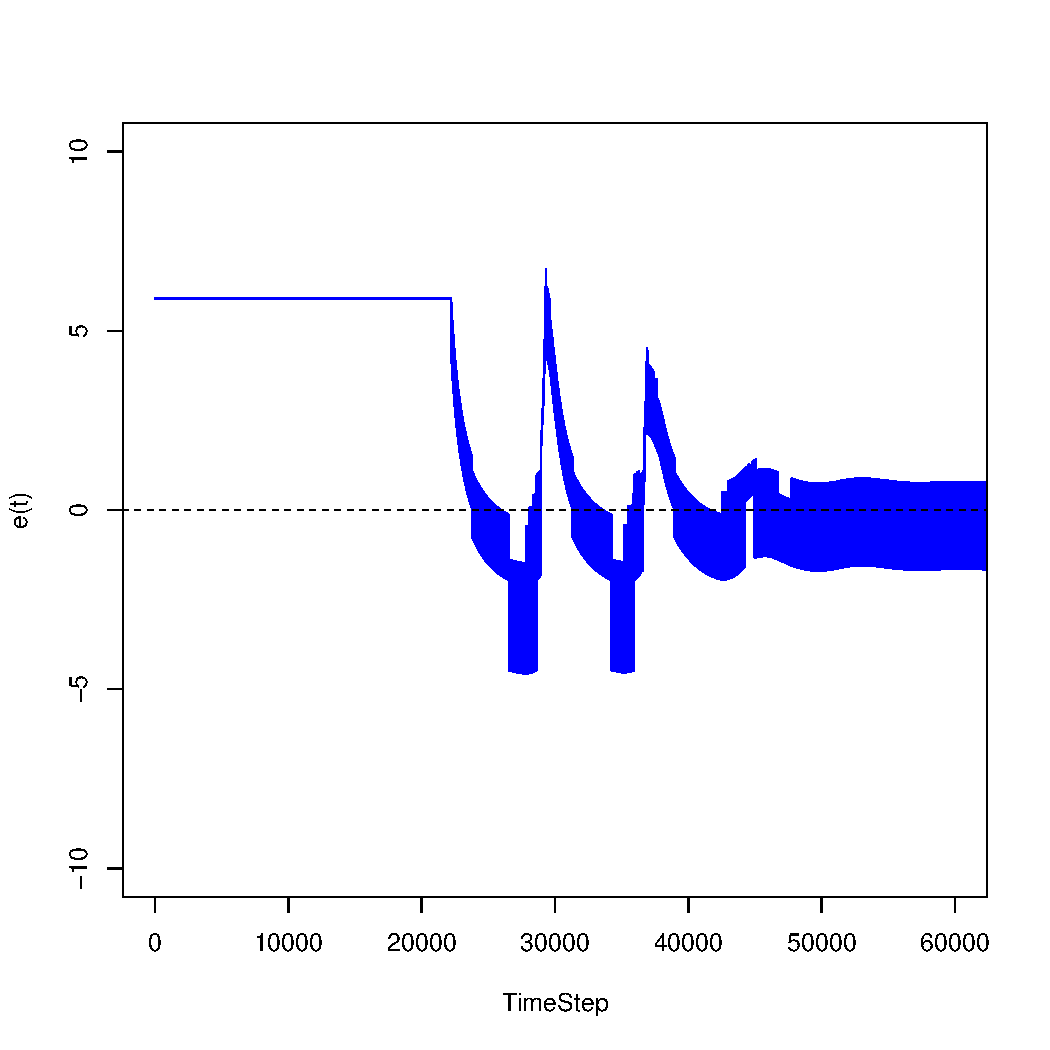
\includegraphics[width=1\hsize]{scenario_5_e_86400_345600_052_0_0.pdf}
%         \subcaption{$e(t)$の変化($K_p = 0.52$)}
%         \label{scenario_5_e_86400_345600_052_0_0}
%         \end{center}
%       \end{minipage}
%       \begin{minipage}{0.5\hsize}
%         \begin{center}
%         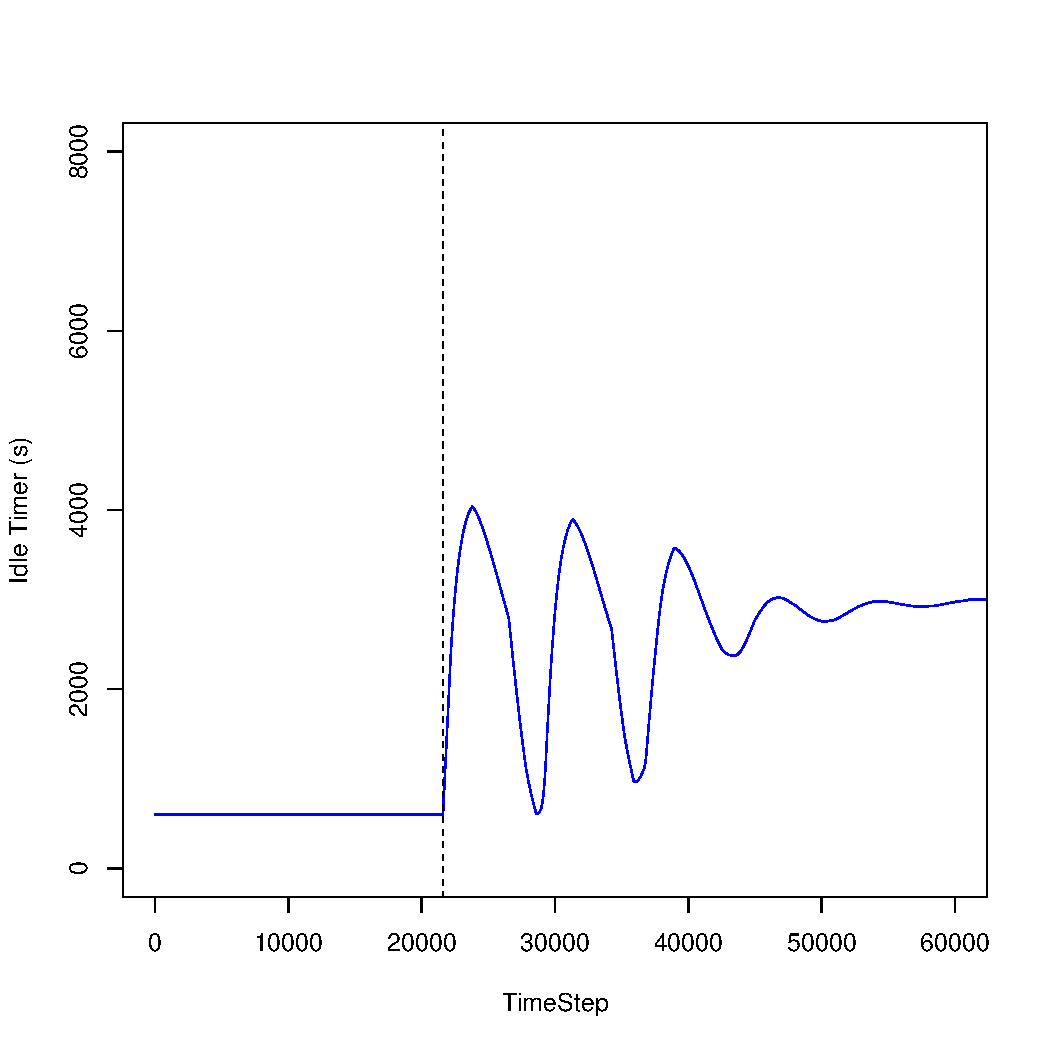
\includegraphics[width=1\hsize]{scenario_5_idleTimer_86400_345600_052_0_0.pdf}
%         \subcaption{IdleTimerの変化($K_p = 0.52$)}
%         \label{scenario_5_idleTimer_86400_345600_052_0_0}
%         \end{center}
%       \end{minipage}\\
%       \begin{minipage}{0.5\hsize}
%         \begin{center}
%         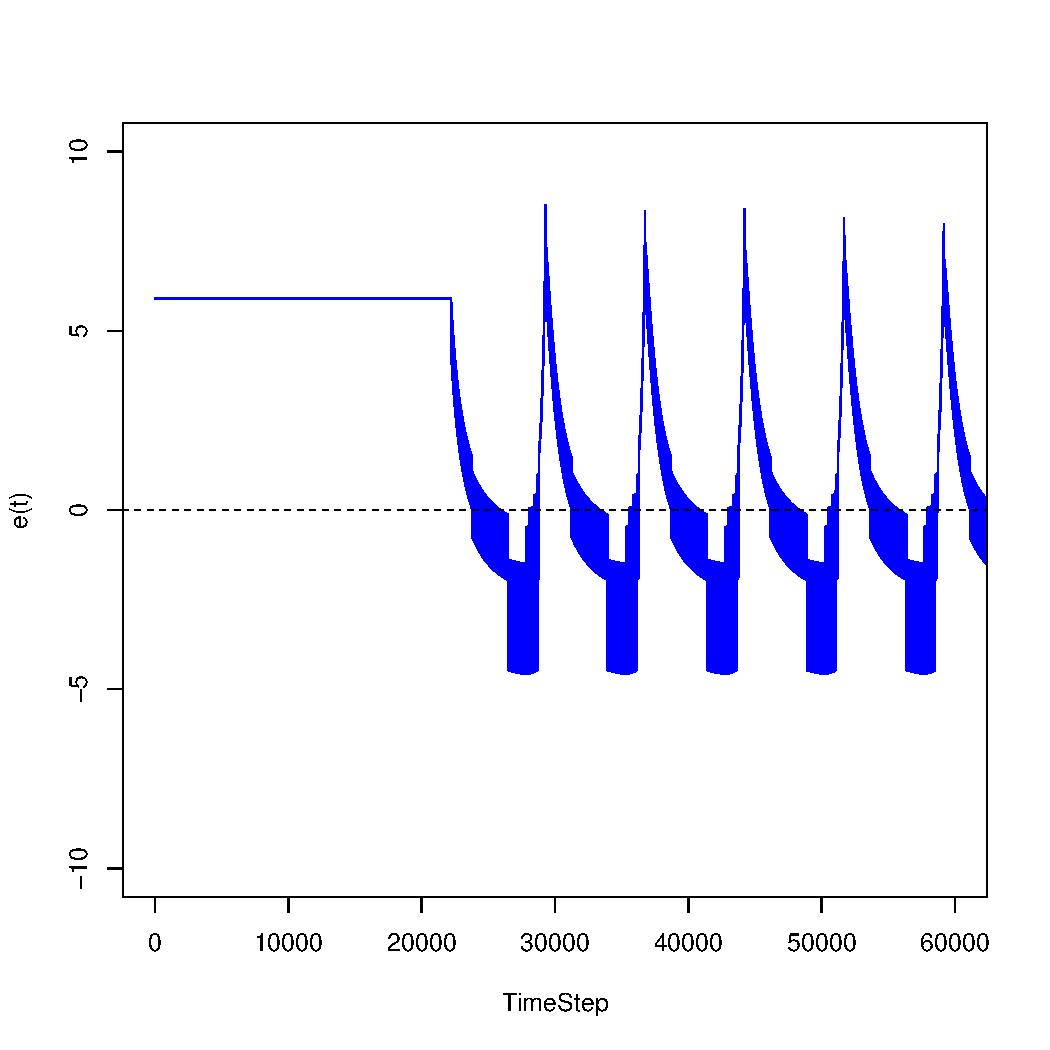
\includegraphics[width=1\hsize]{scenario_5_e_86400_345600_053_0_0.pdf}
%         \subcaption{$e(t)$の変化($K_p = 0.53$)}
%         \label{scenario_5_e_86400_345600_053_0_0}
%         \end{center}
%       \end{minipage}
%       \begin{minipage}{0.5\hsize}
%         \begin{center}
%         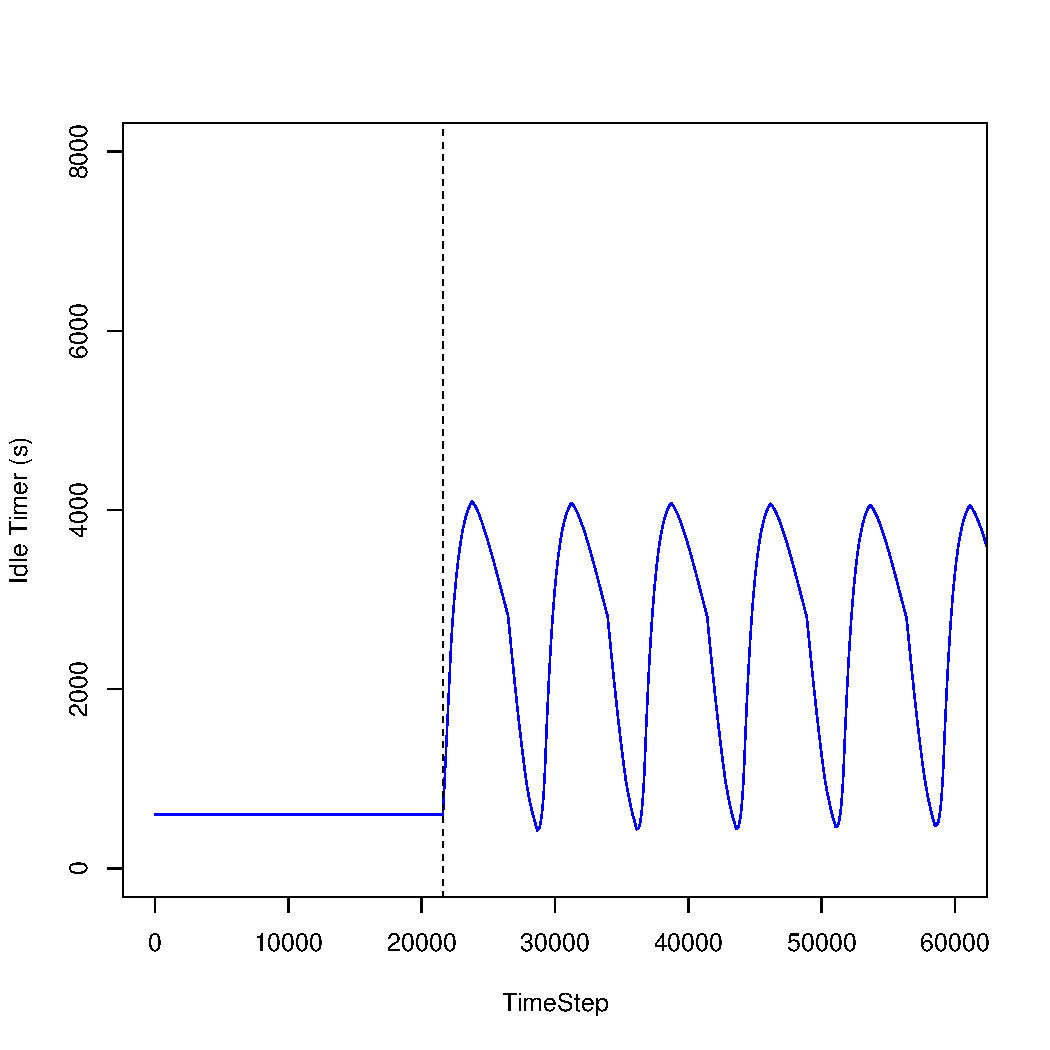
\includegraphics[width=1\hsize]{scenario_5_idleTimer_86400_345600_053_0_0.pdf}
%         \subcaption{IdleTimerの変化($K_p = 0.53$)}
%         \label{scenario_5_idleTimer_86400_345600_053_0_0}
%         \end{center}
%       \end{minipage}
%     \end{tabular}
%     \caption{}
%     \label{result_2}
%   \end{center}
% \end{figure}


以上の結果を用いて、各ゲインの値は以下の表\ref{table:Ziegler-Nichols_setting}のように求まる。
\begin{table}[]
  \centering
  \caption{ジーグラ・ニコルスの限界感度法に基づく設定}
  \label{table:Ziegler-Nichols_setting}
  \begin{tabular}{c|c|c|c|c|c}
    \hline
    制御の種類  & $K_p$ & $K_i$ & $K_d$ &$T_i$&$T_d$  \\\hline \hline
    P & 0.265 & 0 & 0 & - & - \\
    PI & 0.2385 & 0.0000463 & 0 & 6183.5 & -\\
    PID & 0.318 & 0.0000854 & 296.14 & 3725 & 931.25 \\\hline
  \end{tabular}
\end{table}
% \begin{table}[]
%   \centering
%   \caption{ジーグラ・ニコルスの限界感度法に基づく設定}
%   \label{table:Ziegler-Nichols_setting}
%   \begin{tabular}{c|c|c|c}
%     \hline
%     制御の種類  & $K_p$ & $T_i$ & $T_d$ \\\hline \hline
%     P & 0.265 & - & - \\
%     PI & 0.2385 & 6183.5 & - \\
%     PID & 0.318 & 3725 & 931.25 \\\hline
%   \end{tabular}
% \end{table}

\clearpage
表\ref{table:Ziegler-Nichols_setting}に示したP制御の値を$K_p$、$K_i$および$K_d$にそれぞれ設定した場合の評価結果を図\ref{result_p}に示す。
\begin{figure}[htbp]
  \begin{center}
    \begin{tabular}{c}
      \begin{minipage}{0.45\hsize}
        \begin{center}
        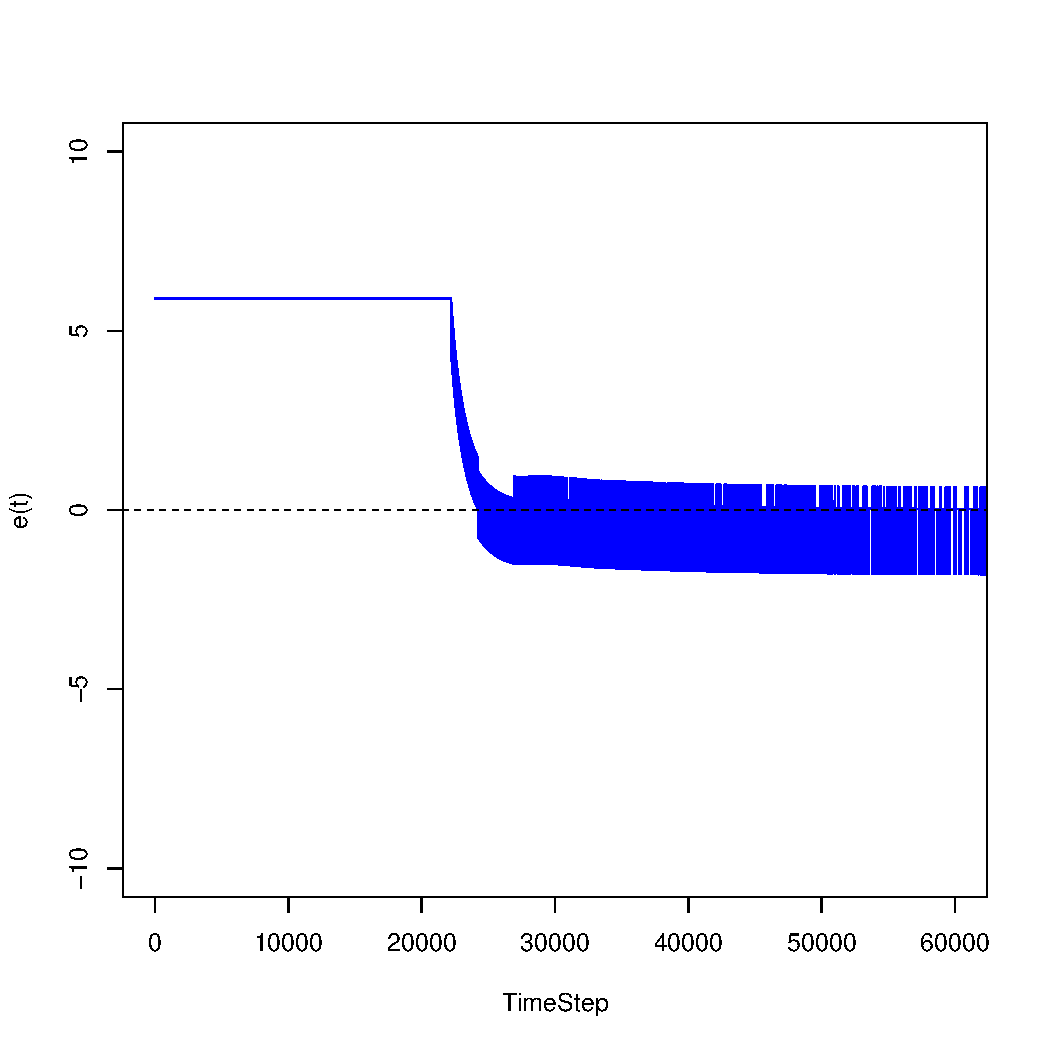
\includegraphics[width=1\hsize]{scenario_5_e_86400_345600_0-265_0_0.pdf}
        \subcaption{$e(t)$の変化($K_p = 0.265、K_i = 0、K_d = 0$)}
        \label{scenario_5_e_86400_345600_0-265_0_0}
        \end{center}
      \end{minipage}
      \begin{minipage}{0.45\hsize}
        \begin{center}
        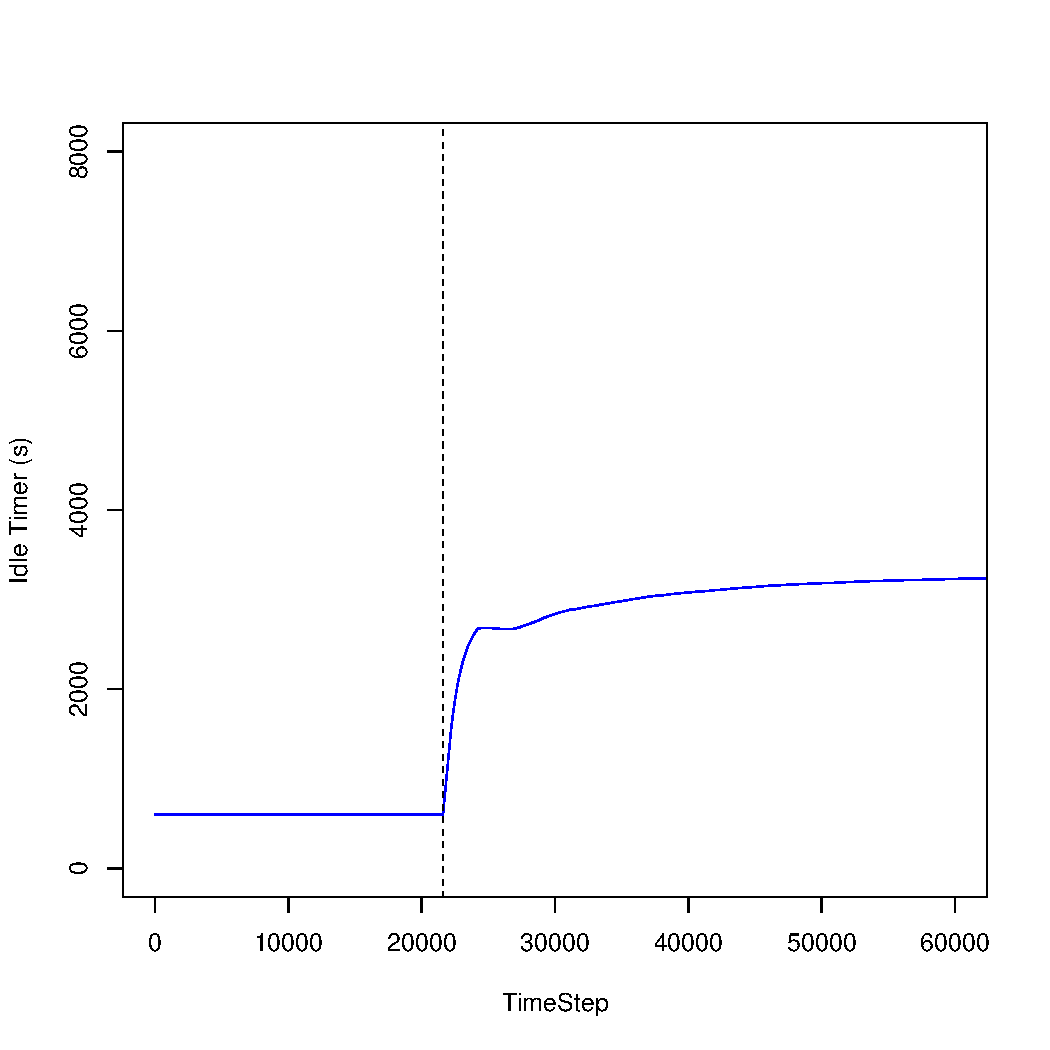
\includegraphics[width=1\hsize]{scenario_5_idleTimer_86400_345600_0-265_0_0.pdf}
        \subcaption{IdleTimerの変化($K_p = 0.265、K_i = 0、K_d = 0$)}
        \label{scenario_5_idleTimer_86400_345600_0-265_0_0}
        \end{center}
      \end{minipage}\\
      \begin{minipage}{0.45\hsize}
        \begin{center}
        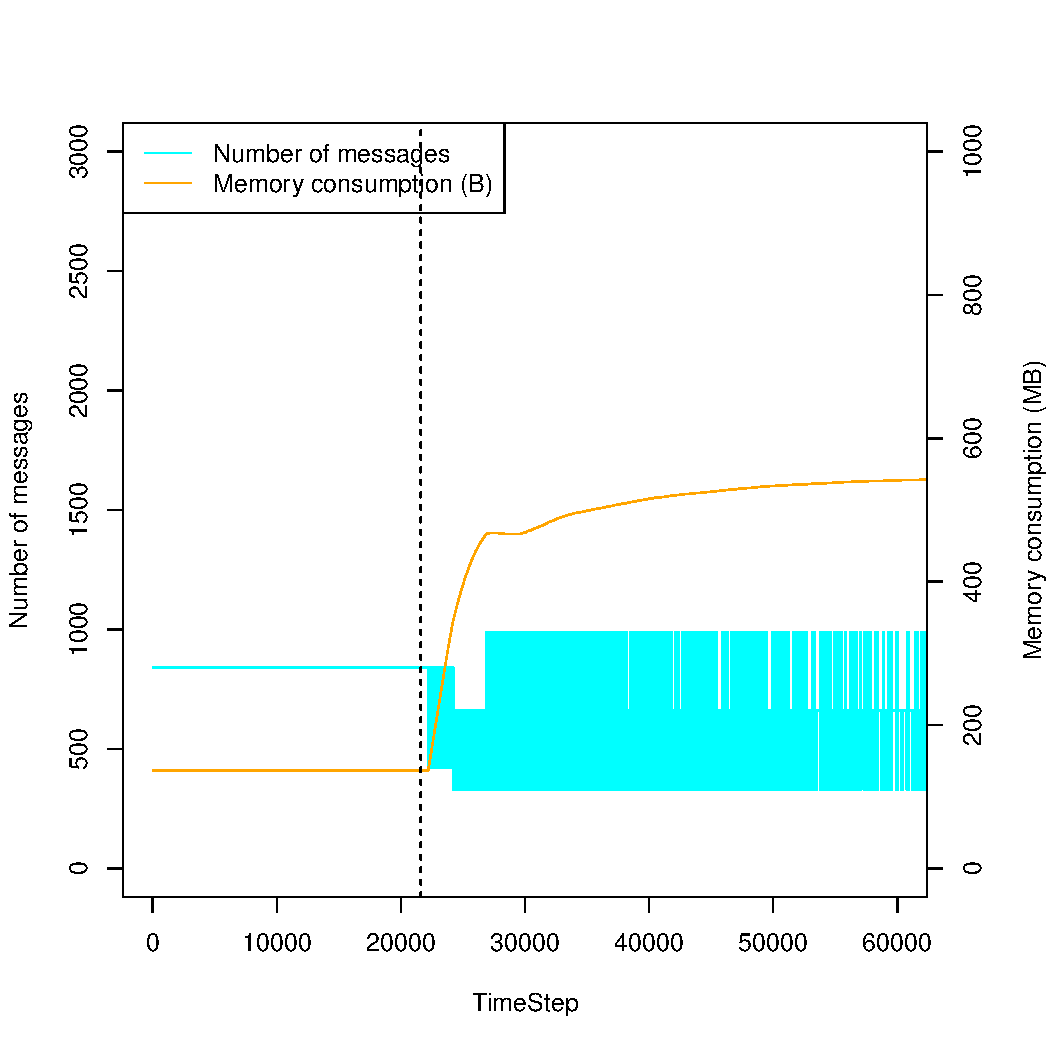
\includegraphics[width=1\hsize]{scenario_5_signaling_and_memoryload_vs_timeStep_86400_345600_0-265_0_0.pdf}
        \subcaption{CPU負荷とメモリ使用量の変化($K_p = 0.265、K_i = 0、K_d = 0$)}
        \label{scenario_5_signaling_and_memoryload_vs_timeStep_86400_345600_0-265_0_0}
        \end{center}
      \end{minipage}
      \begin{minipage}{0.45\hsize}
        \begin{center}
        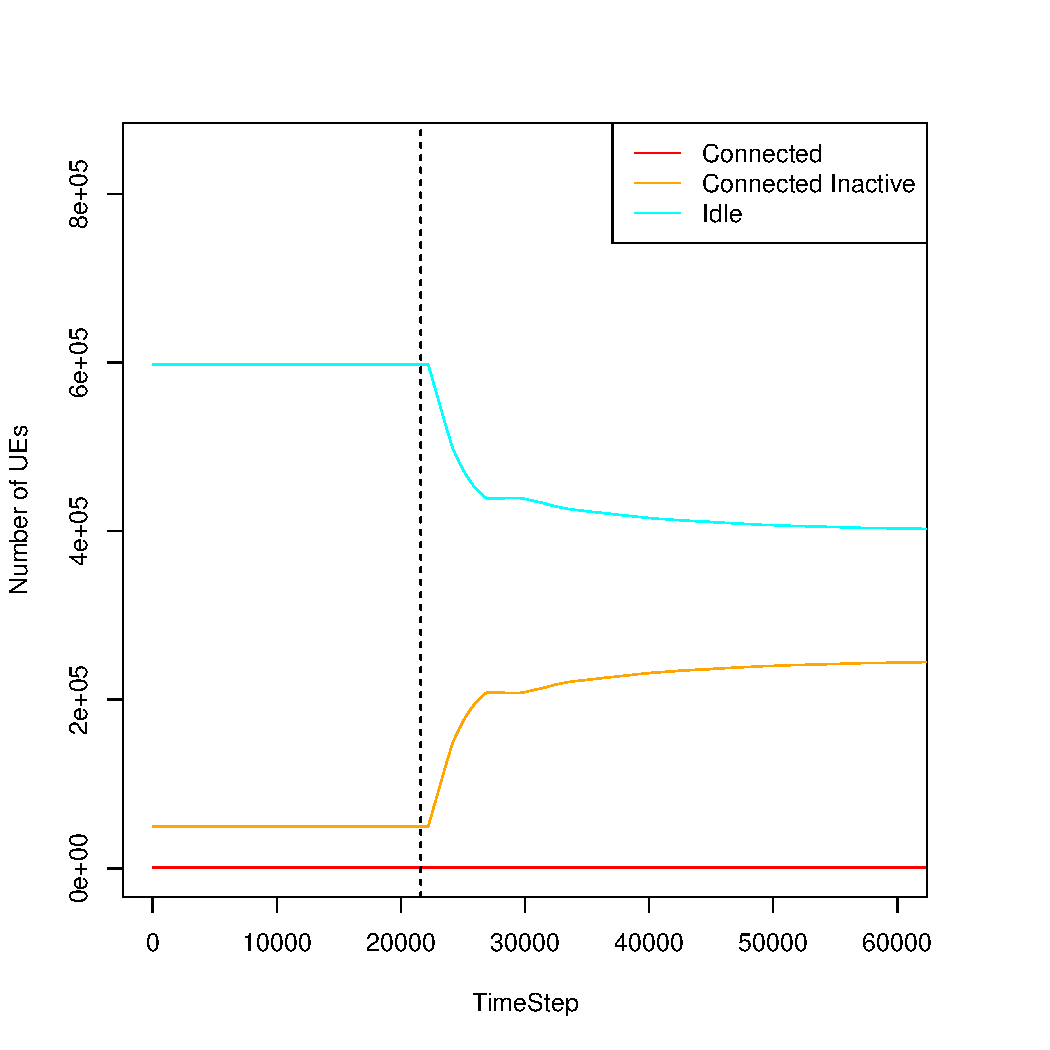
\includegraphics[width=1\hsize]{scenario_5_stateBreakdown_86400_345600_0-265_0_0.pdf}
        \subcaption{各状態にあるUE台数の変化($K_p = 0.265、K_i = 0、K_d = 0$)}
        \label{scenario_5_stateBreakdown_86400_345600_0-265_0_0}
        \end{center}
      \end{minipage}
    \end{tabular}
    \caption{}
    \label{result_p}
  \end{center}
\end{figure}
\clearpage
表\ref{table:Ziegler-Nichols_setting}に示したPI制御の値を$K_p$、$K_i$および$K_d$にそれぞれ設定した場合の評価結果を図\ref{result_pi}に示す。
\begin{figure}[htbp]
  \begin{center}
    \begin{tabular}{c}
      \begin{minipage}{0.45\hsize}
        \begin{center}
        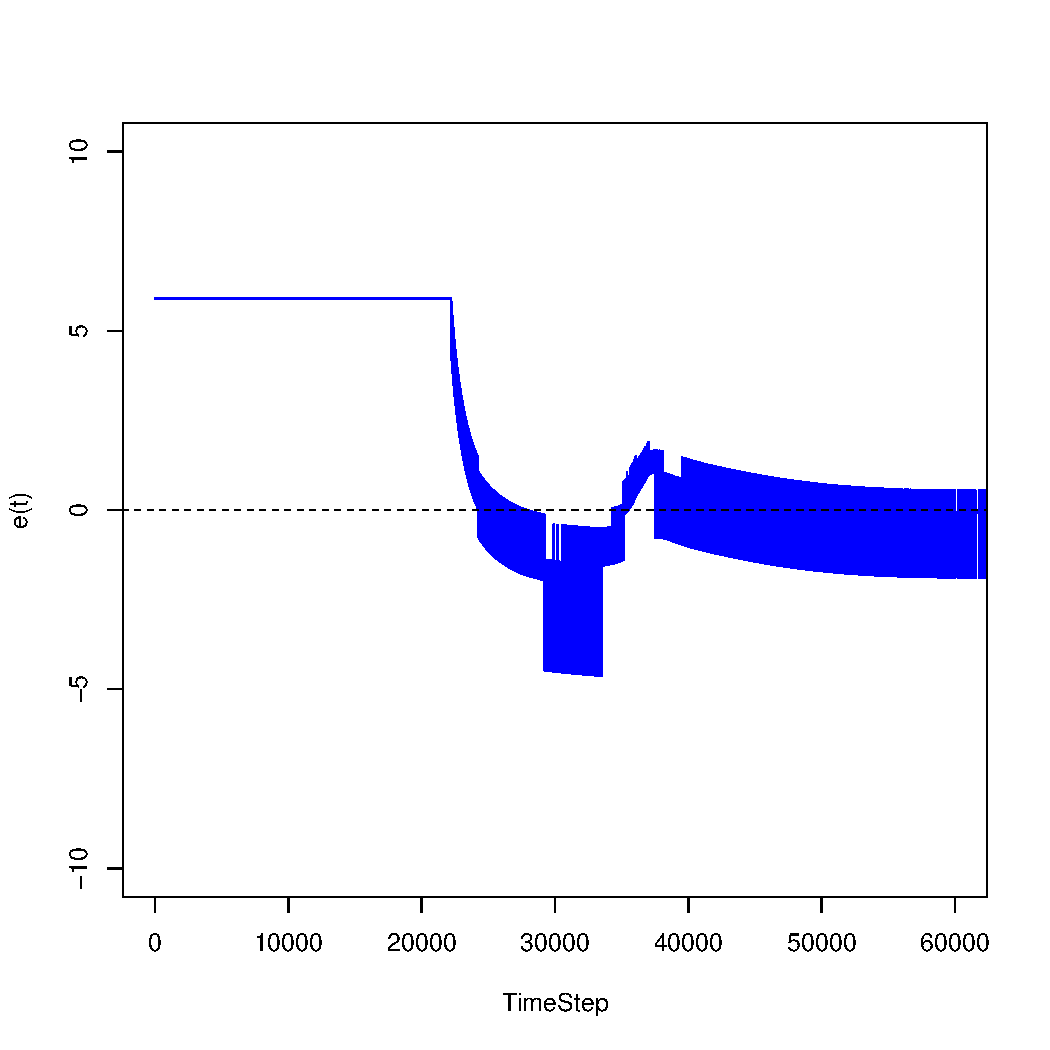
\includegraphics[width=1\hsize]{scenario_5_e_86400_345600_0-2385_0-0000463_0.pdf}
        \subcaption{$e(t)$の変化($K_p = 0.2385、K_i = 0.0000463、K_d = 0$)}
        \label{scenario_5_e_86400_345600_0-2385_0-0000463_0}
        \end{center}
      \end{minipage}
      \begin{minipage}{0.45\hsize}
        \begin{center}
        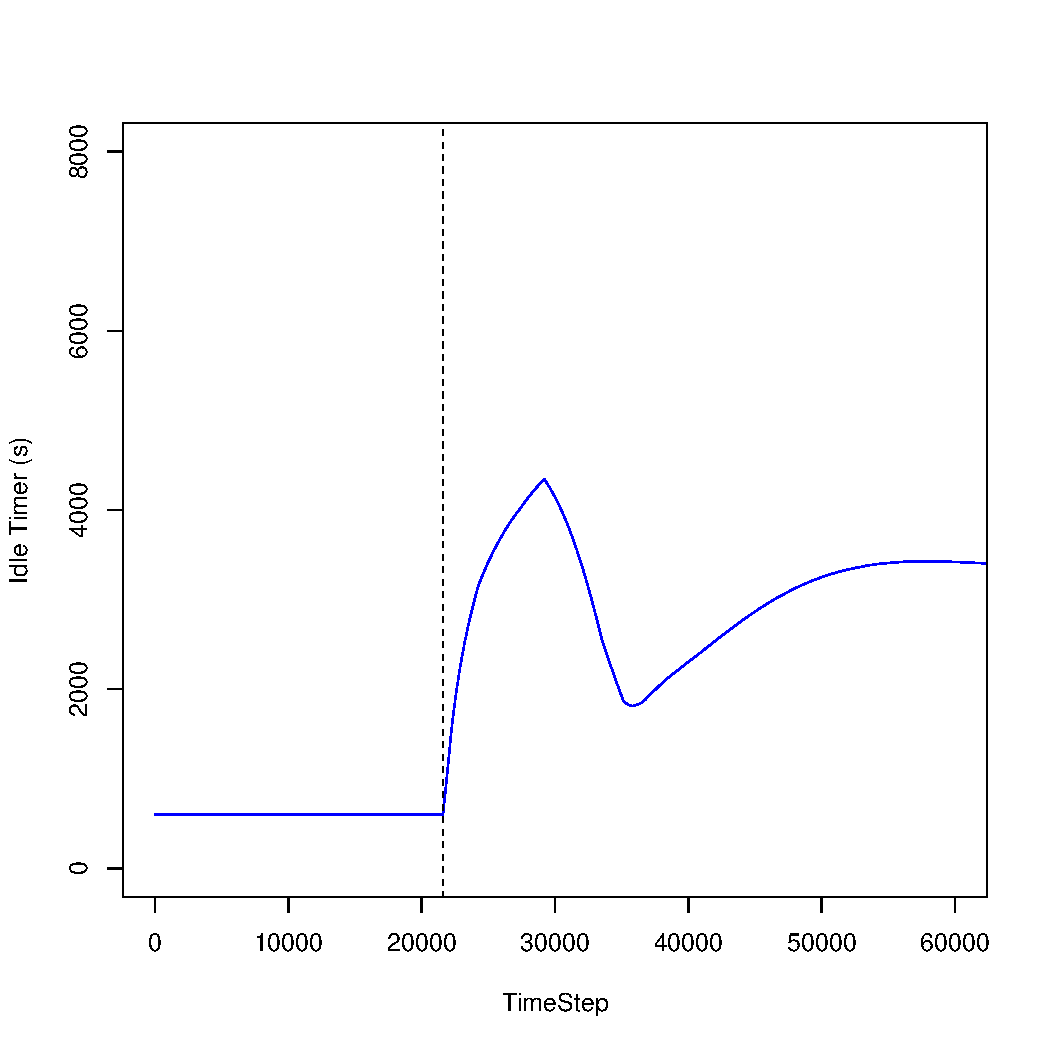
\includegraphics[width=1\hsize]{scenario_5_idleTimer_86400_345600_0-2385_0-0000463_0.pdf}
        \subcaption{IdleTimerの変化($K_p = 0.2385、K_i = 0.0000463、K_d = 0$)}
        \label{scenario_5_idleTimer_86400_345600_0-2385_0-0000463_0}
        \end{center}
      \end{minipage}\\
      \begin{minipage}{0.45\hsize}
        \begin{center}
        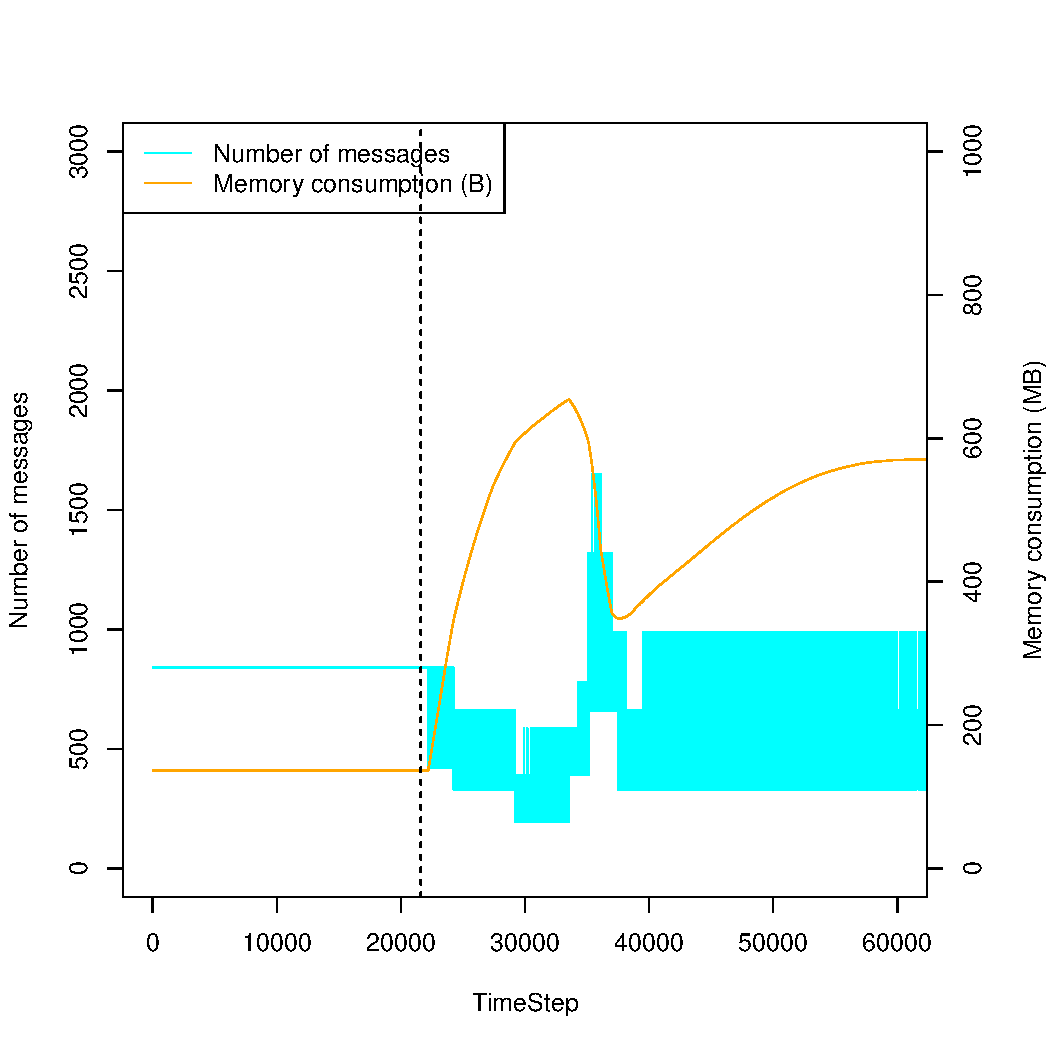
\includegraphics[width=1\hsize]{scenario_5_signaling_and_memoryload_vs_timeStep_86400_345600_0-2385_0-0000463_0.pdf}
        \subcaption{CPU負荷とメモリ使用量の変化($K_p = 0.2385、K_i = 0.0000463、K_d = 0$)}
        \label{scenario_5_signaling_and_memoryload_vs_timeStep_86400_345600_0-2385_0-0000463_0}
        \end{center}
      \end{minipage}
      \begin{minipage}{0.45\hsize}
        \begin{center}
        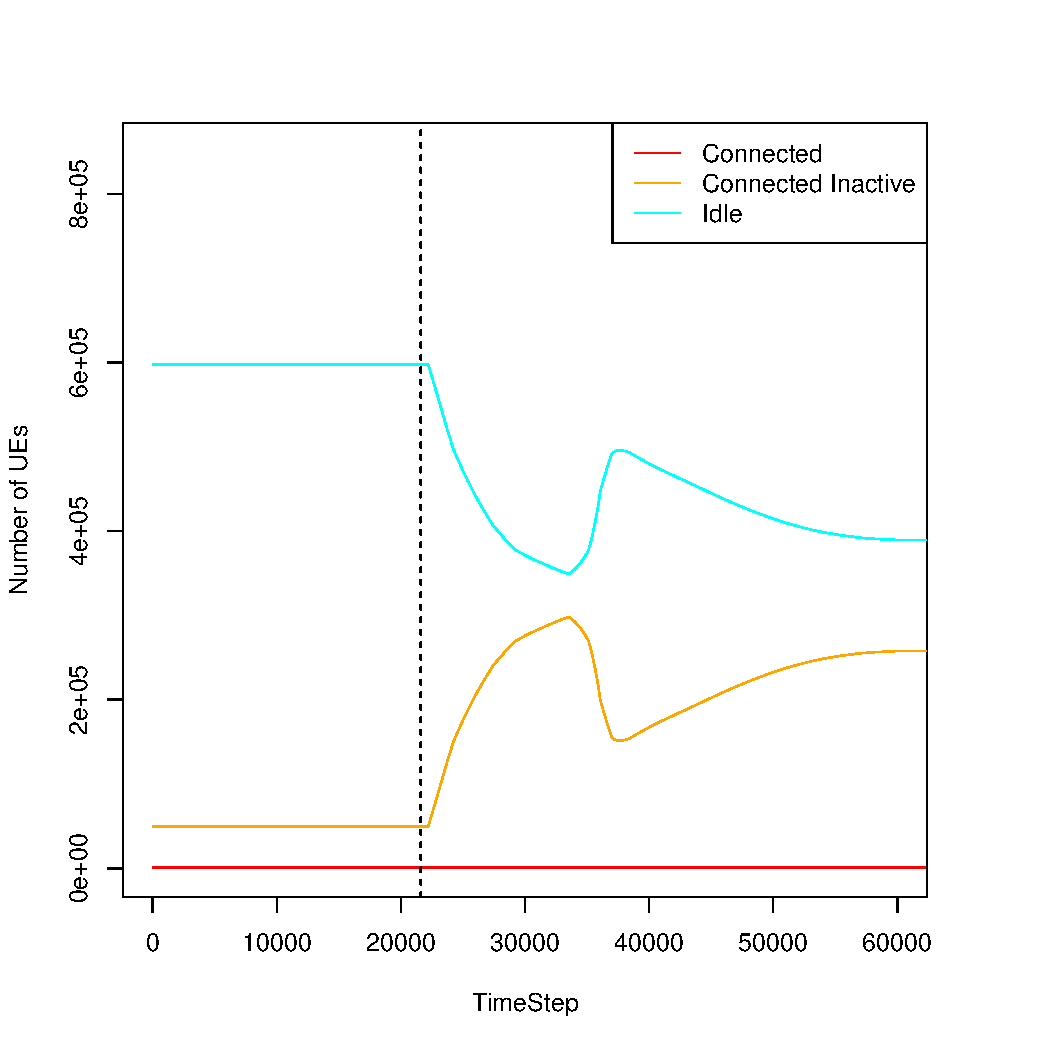
\includegraphics[width=1\hsize]{scenario_5_stateBreakdown_86400_345600_0-2385_0-0000463_0.pdf}
        \subcaption{各状態にあるUE台数の変化($K_p = 0.2385、K_i = 0.0000463、K_d = 0$)}
        \label{scenario_5_stateBreakdown_86400_345600_0-2385_0-0000463_0}
        \end{center}
      \end{minipage}
    \end{tabular}
    \caption{}
    \label{result_pi}
  \end{center}
\end{figure}
\clearpage
表\ref{table:Ziegler-Nichols_setting}に示したPID制御の値を$K_p$、$K_i$および$K_d$にそれぞれ設定した場合の評価結果を図\ref{result_pid}に示す。
\begin{figure}[htbp]
  \begin{center}
    \begin{tabular}{c}
      \begin{minipage}{0.45\hsize}
        \begin{center}
        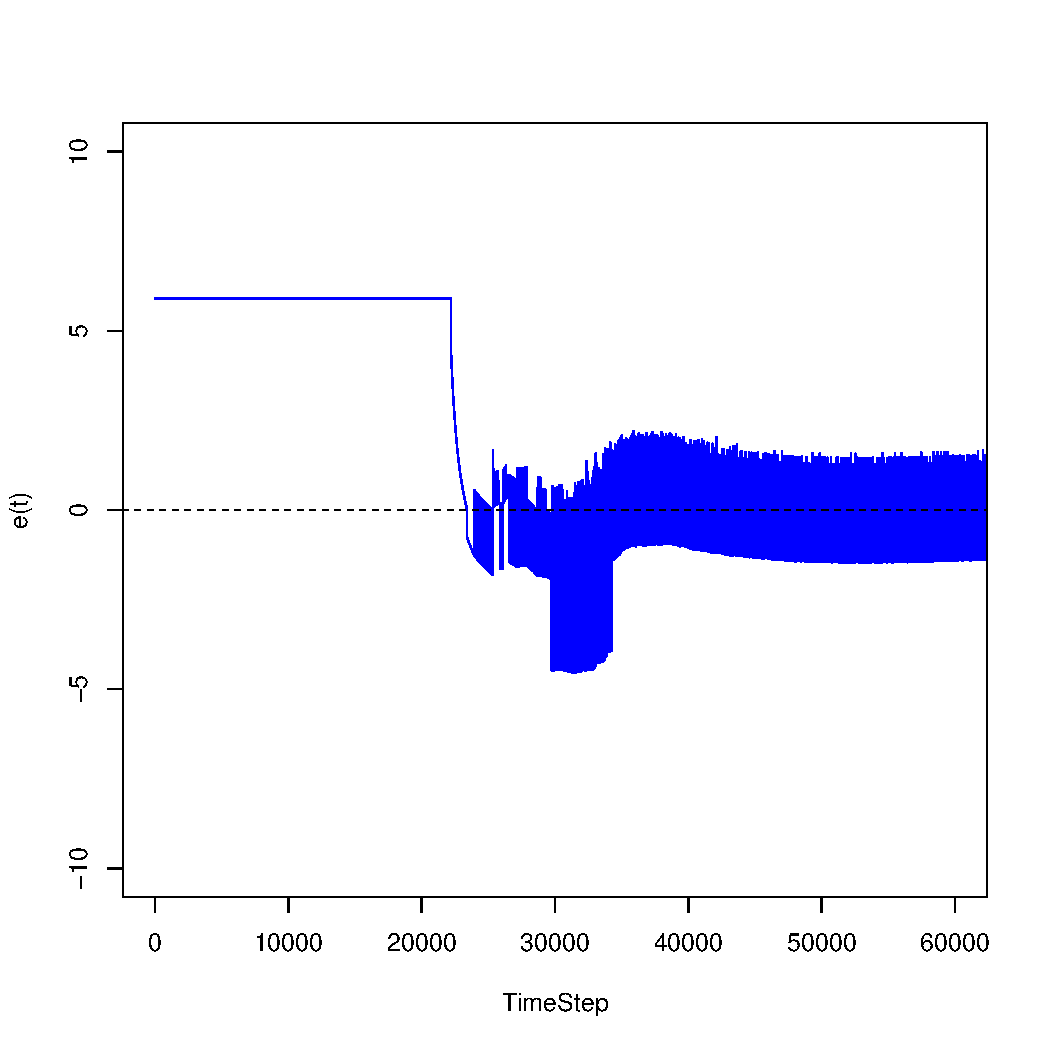
\includegraphics[width=1\hsize]{scenario_5_e_86400_345600_0-318_0-0000854_296-14.pdf}
        \subcaption{$e(t)$の変化($K_p = 0.318、K_i = 0.0000854、K_d = 296.14$)}
        \label{scenario_5_e_86400_345600_0-318_0-0000854_296-14}
        \end{center}
      \end{minipage}
      \begin{minipage}{0.45\hsize}
        \begin{center}
        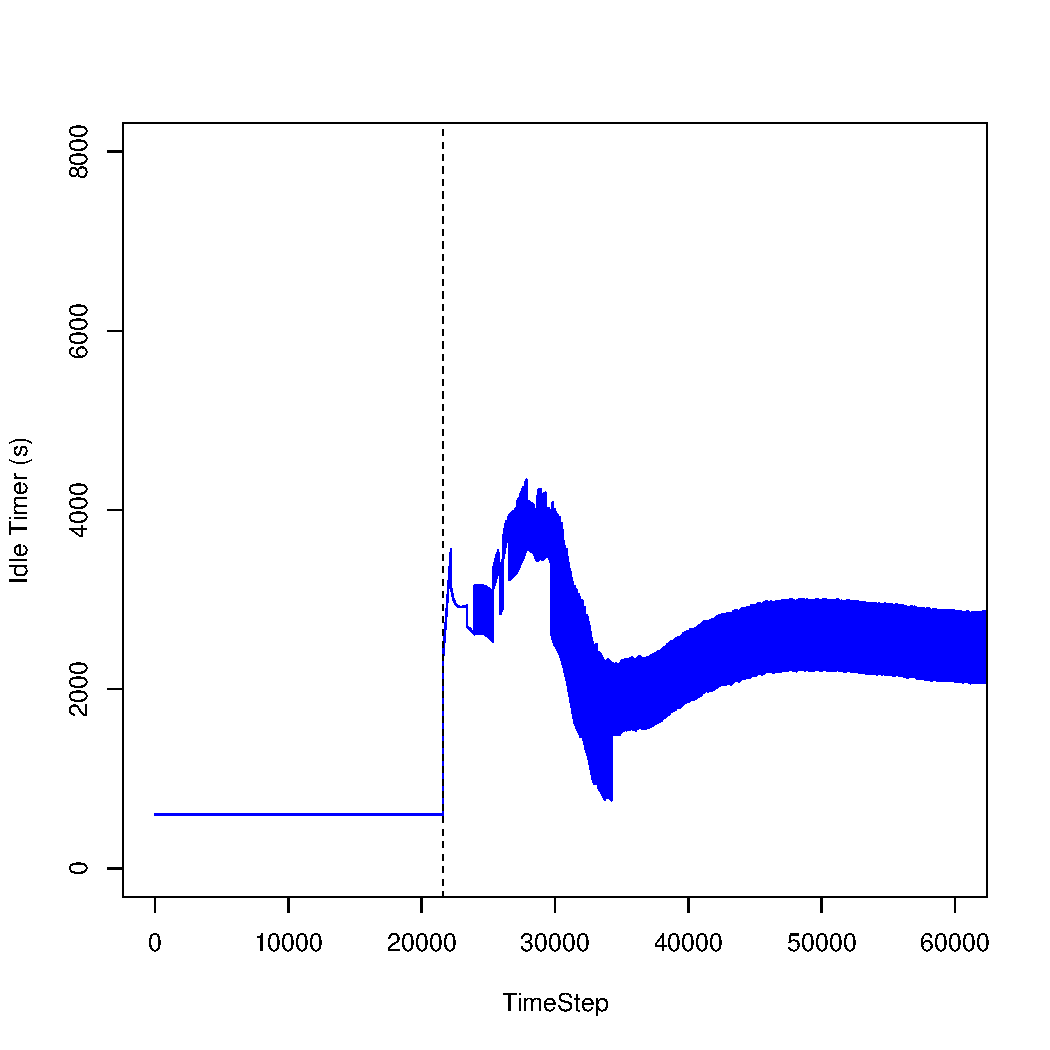
\includegraphics[width=1\hsize]{scenario_5_idleTimer_86400_345600_0-318_0-0000854_296-14.pdf}
        \subcaption{IdleTimerの変化($K_p = 0.318、K_i = 0.0000854、K_d = 296.14$)}
        \label{scenario_5_idleTimer_86400_345600_0-318_0-0000854_296-14}
        \end{center}
      \end{minipage}\\
      \begin{minipage}{0.45\hsize}
        \begin{center}
        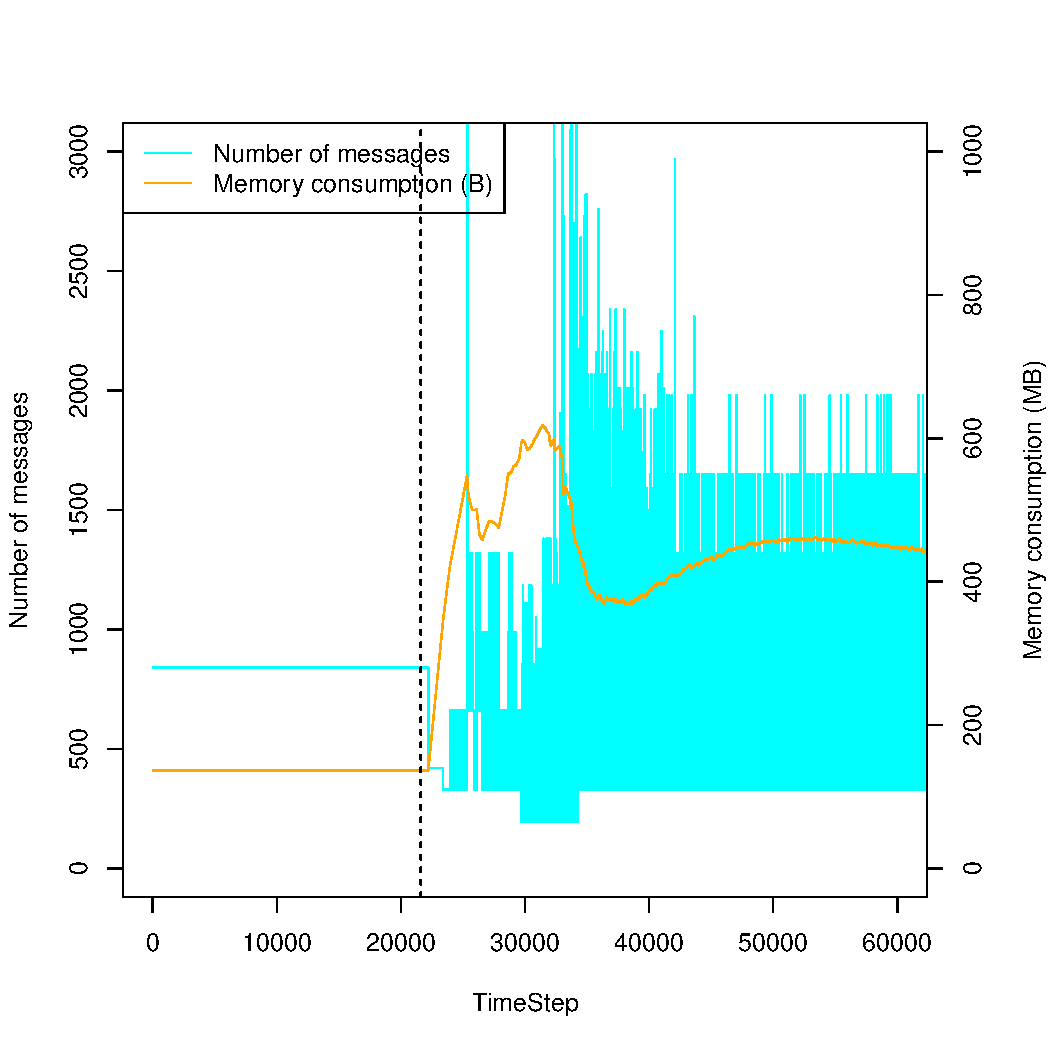
\includegraphics[width=1\hsize]{scenario_5_signaling_and_memoryload_vs_timeStep_86400_345600_0-318_0-0000854_296-14.pdf}
        \subcaption{CPU負荷とメモリ使用量の変化($K_p = 0.318、K_i = 0.0000854、K_d = 296.14$)}
        \label{scenario_5_signaling_and_memoryload_vs_timeStep_86400_345600_0-318_0-0000854_296-14}
        \end{center}
      \end{minipage}
      \begin{minipage}{0.45\hsize}
        \begin{center}
        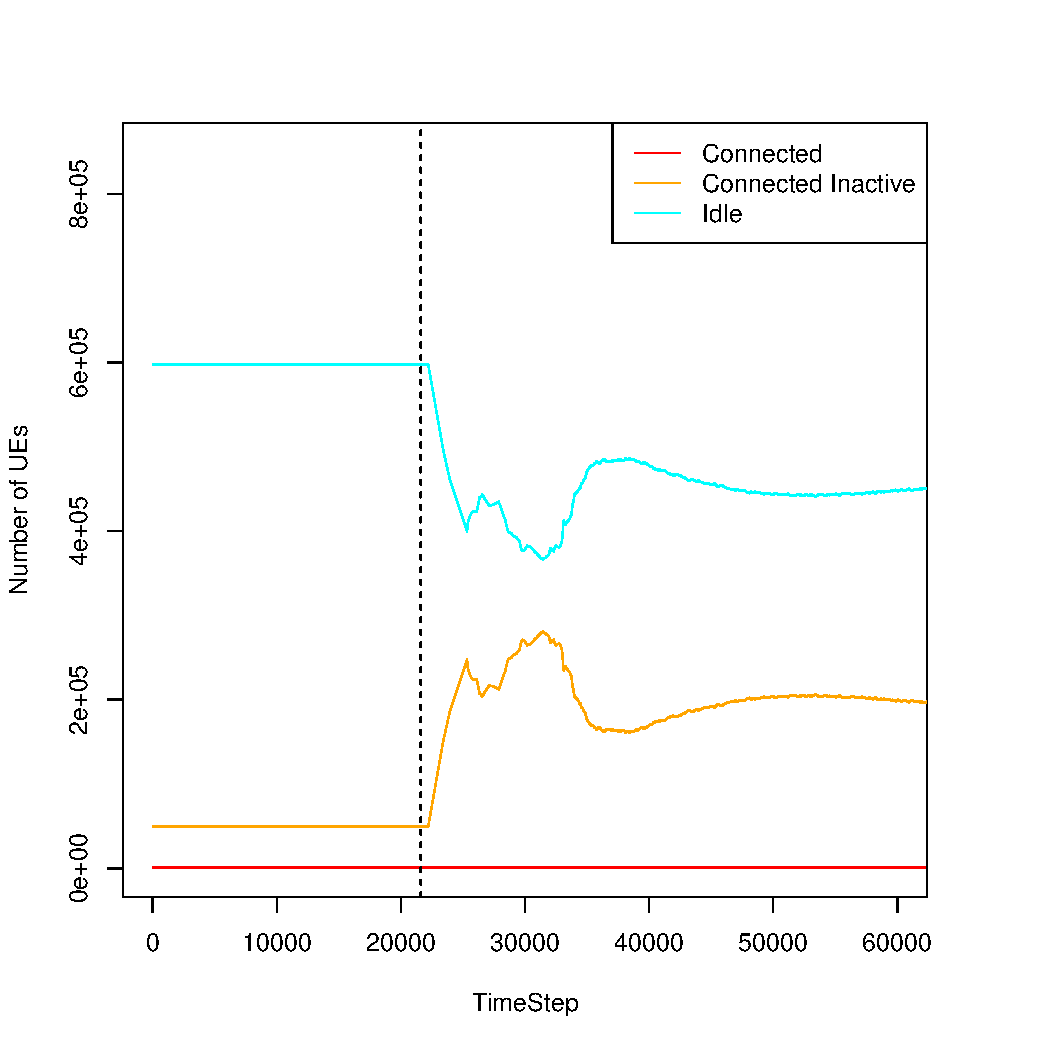
\includegraphics[width=1\hsize]{scenario_5_stateBreakdown_86400_345600_0-318_0-0000854_296-14.pdf}
        \subcaption{各状態にあるUE台数の変化($K_p = 0.318、K_i = 0.0000854、K_d = 296.14$)}
        \label{scenario_5_stateBreakdown_86400_345600_0-318_0-0000854_296-14}
        \end{center}
      \end{minipage}
    \end{tabular}
    \caption{}
    \label{result_pid}
  \end{center}
\end{figure}
\clearpage
表\ref{table:Ziegler-Nichols_setting}に示したPID制御の値を、$K_p$および$K_d$にそれぞれ設定し、$K_i$に0を設定した場合の評価結果を図\ref{result_pd}に示す。
\begin{figure}[htbp]
  \begin{center}
    \begin{tabular}{c}
      \begin{minipage}{0.45\hsize}
        \begin{center}
        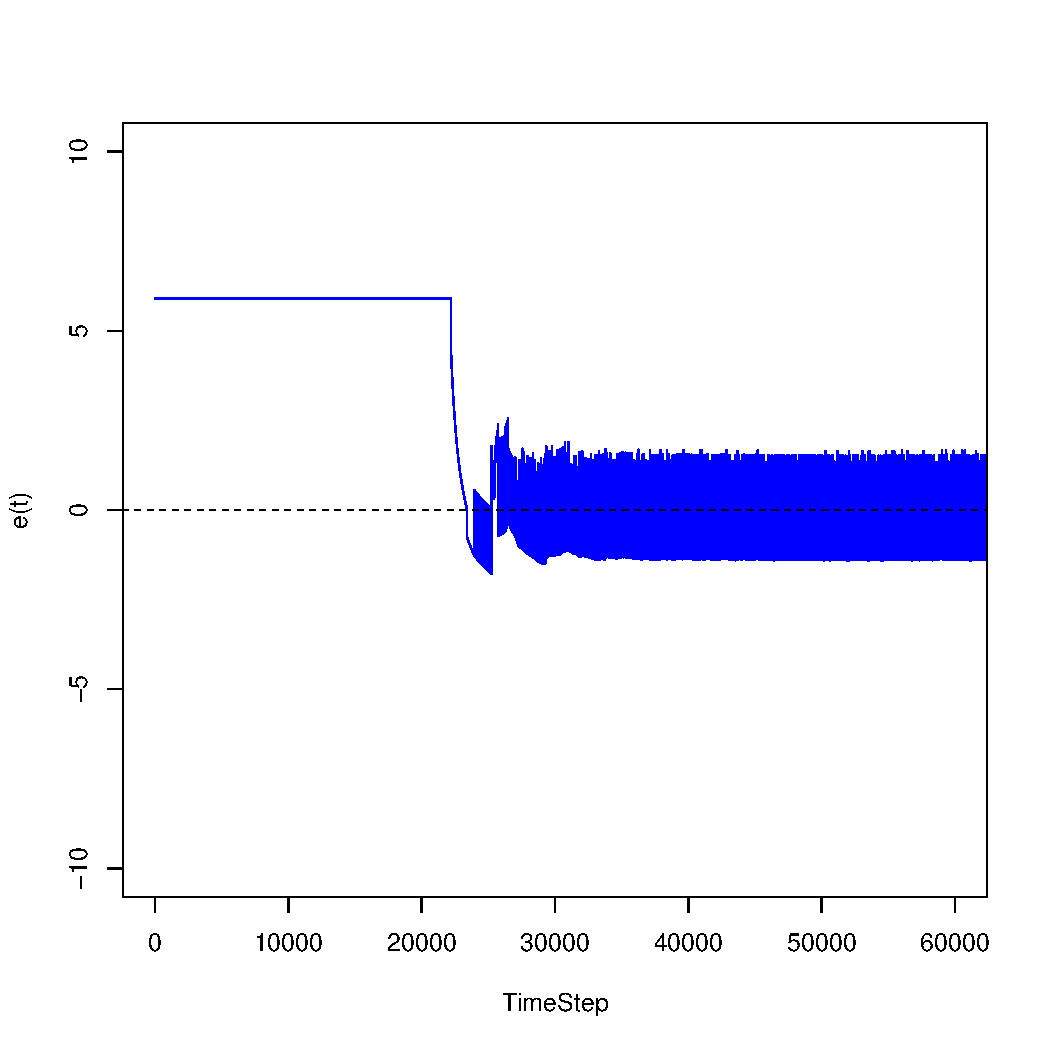
\includegraphics[width=1\hsize]{scenario_5_e_86400_345600_0-318_0_296-14.pdf}
        \subcaption{$e(t)$の変化($K_p = 0.318、K_i = 0、K_d = 296.14$)}
        \label{scenario_5_e_86400_345600_0-318_0_296-14}
        \end{center}
      \end{minipage}
      \begin{minipage}{0.45\hsize}
        \begin{center}
        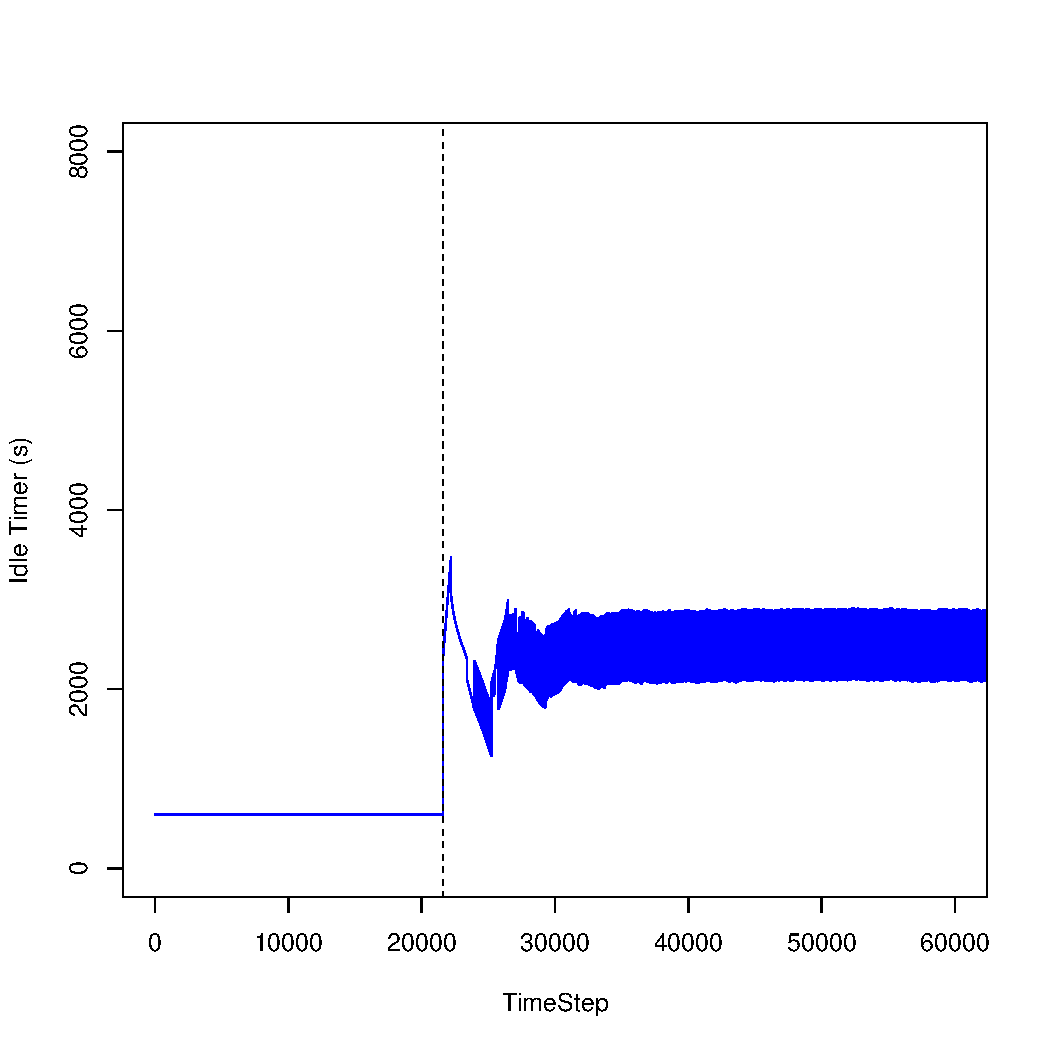
\includegraphics[width=1\hsize]{scenario_5_idleTimer_86400_345600_0-318_0_296-14.pdf}
        \subcaption{IdleTimerの変化($K_p = 0.318、K_i = 0、K_d = 296.14$)}
        \label{scenario_5_idleTimer_86400_345600_0-318_0_296-14}
        \end{center}
      \end{minipage}\\
      \begin{minipage}{0.45\hsize}
        \begin{center}
        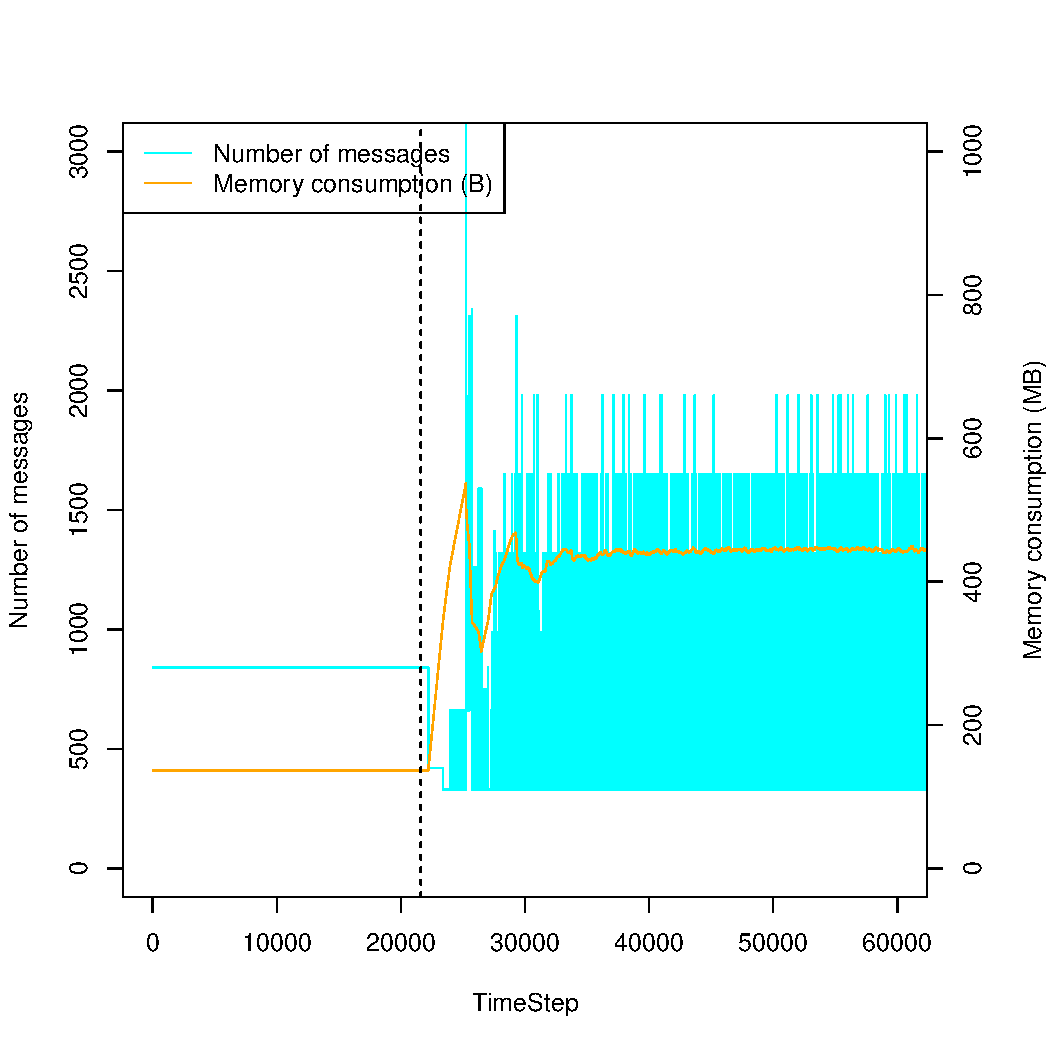
\includegraphics[width=1\hsize]{scenario_5_signaling_and_memoryload_vs_timeStep_86400_345600_0-318_0_296-14.pdf}
        \subcaption{CPU負荷とメモリ使用量の変化($K_p = 0.318、K_i = 0、K_d = 296.14$)}
        \label{scenario_5_signaling_and_memoryload_vs_timeStep_86400_345600_0-318_0_296-14}
        \end{center}
      \end{minipage}
      \begin{minipage}{0.45\hsize}
        \begin{center}
        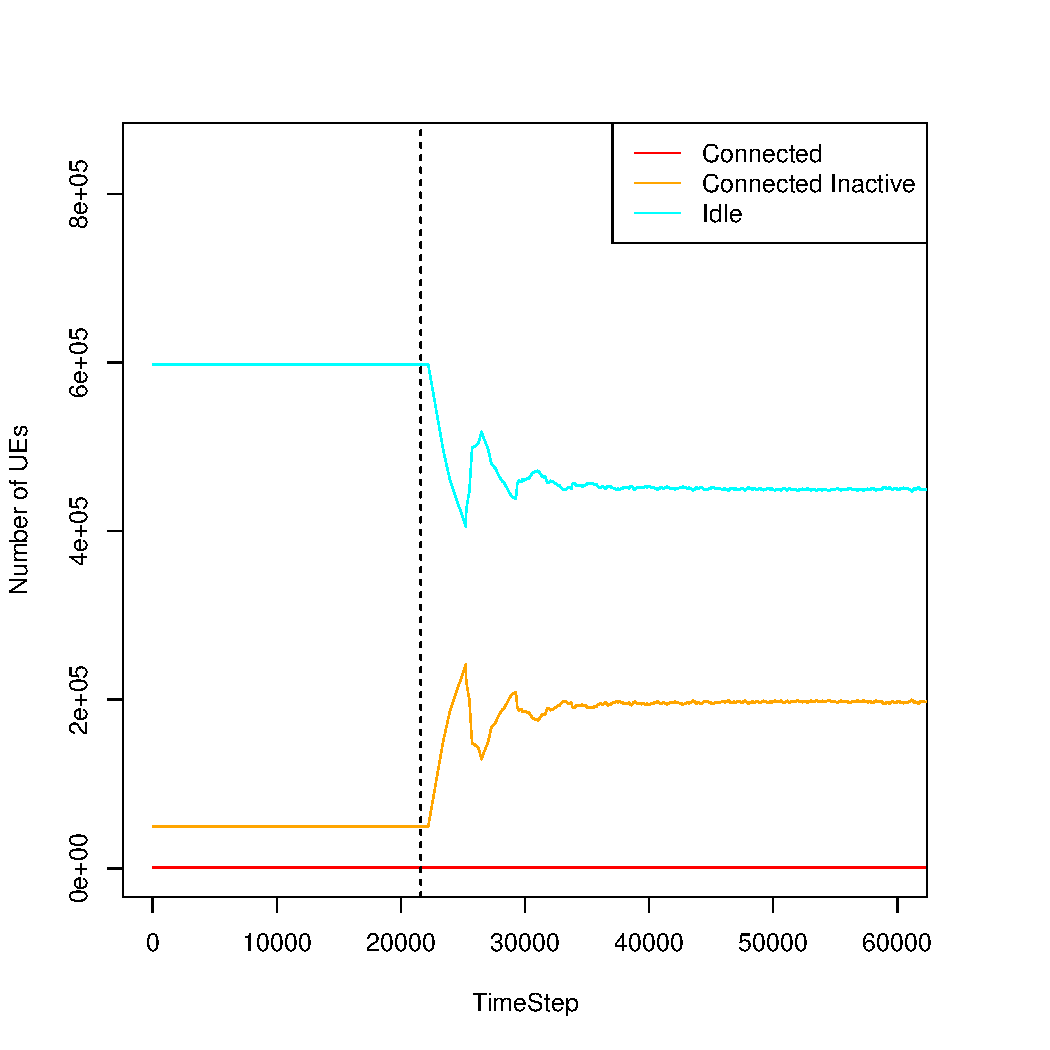
\includegraphics[width=1\hsize]{scenario_5_stateBreakdown_86400_345600_0-318_0_296-14.pdf}
        \subcaption{各状態にあるUE台数の変化($K_p = 0.318、K_i = 0、K_d = 296.14$)}
        \label{scenario_5_stateBreakdown_86400_345600_0-318_0_296-14}
        \end{center}
      \end{minipage}
    \end{tabular}
    \caption{}
    \label{result_pd}
  \end{center}
\end{figure}
\clearpage
以上の図\ref{result_p}、\ref{result_pi}図\ref{result_pid}を比較すると、図\ref{result_p}に示したP制御が最も制御が安定していることがわかる。また、$E(t)$が0に収束するまでの時間も最も短くなっている。以上の結果より、比例ゲインに 0.265 を設定したP制御がIdleタイマの制御に最も適していると言える。

一方で、PI制御は、P制御と比較して良い結果が得られなかった。積分ゲインを利用しても制御が改善しなかった理由は、比例ゲインのみで制御した場合に発生するオフセット(定常偏差)が小さいことがあげられる。オフセットとは、定常状態の時に出力値と目標値の差である。一般的にオフセットを0に収束させるために積分制御が用いられるが、今回評価しているIdleタイマの制御では、元々オフセットが小さい。よって、積分制御を導入するのメリットが小さくなっている。

また、PID制御では、微分ゲインを利用することにより、偏差発生から定常状態に至るまでの過渡応答特性を改善することができた。これは一般的に微分ゲインを導入するメリットの一つである。しかし、一般的に、微分制御は、「対象の変化」ではなく、ノイズにより過敏に反応する危険性がある。本評価では、離散的な負荷の変動が発生しているため、Idleタイマの制御が不安的になっている。

\clearpage
\section{実用PID制御についての調査}
第\ref{gigura}章の評価において、PID制御の微分動作が離散的な負荷の変動の影響を受けやすいため、今回の評価においては制御が不安定になることがわかった。通常の微分(完全微分)を用いて動作するPID制御のことを``理想PID制御"とよび、以下の式(\ref{eq:PID_ideal1})で表せる。以下の図\ref{pid_ideal_block}に、理想PID制御のブロック図を示す。
\begin{eqnarray}
  u(t) &=& K_p \cdot e(t) + K_i \cdot \int_0^t e(\tau) d\tau + K_d \cdot \frac{de(t)}{dt}
  \label{eq:PID_ideal1}
\end{eqnarray}
ここで、積分ゲイン$K_i = K_p / T_i$、微分ゲイン$K_d = K_p \cdot T_d$と表し、式(\ref{eq:PID_ideal1})に代入すると、式(\ref{eq:PID_ideal2})になる。
\begin{eqnarray}
  u(t) &=& K_p \cdot (e(t) + \frac{1}{T_i} \cdot \int_0^t e(\tau) d\tau +  T_d \cdot \frac{de(t)}{dt})
  \label{eq:PID_ideal2}
\end{eqnarray}
式(\ref{eq:PID_ideal2})をラプラス変換すると式(\ref{eq:PID_ideal3})になり、伝達関数$C(s)$は式(\ref{eq:PID_ideal4})となる。
\begin{eqnarray}
  \mathcal{L}[u(t)] &=& \mathcal{L}[K_p \cdot (e(t) + \frac{1}{T_i} \cdot \int_0^t e(\tau) d\tau +  T_d \cdot \frac{de(t)}{dt})] \nonumber\\
  U(s) &=& K_p \cdot (1 + \frac{1}{T_i \cdot s}  +  T_d \cdot s) \cdot E(s)
  \label{eq:PID_ideal3}
\end{eqnarray}
\begin{eqnarray}
  C(s) &=& \frac{U(s)}{E(s)} = K_p \cdot (1 + \frac{1}{T_i \cdot s}  +  T_d \cdot s)
  \label{eq:PID_ideal4}
\end{eqnarray}

\begin{figure}[htbp]
  \centering
  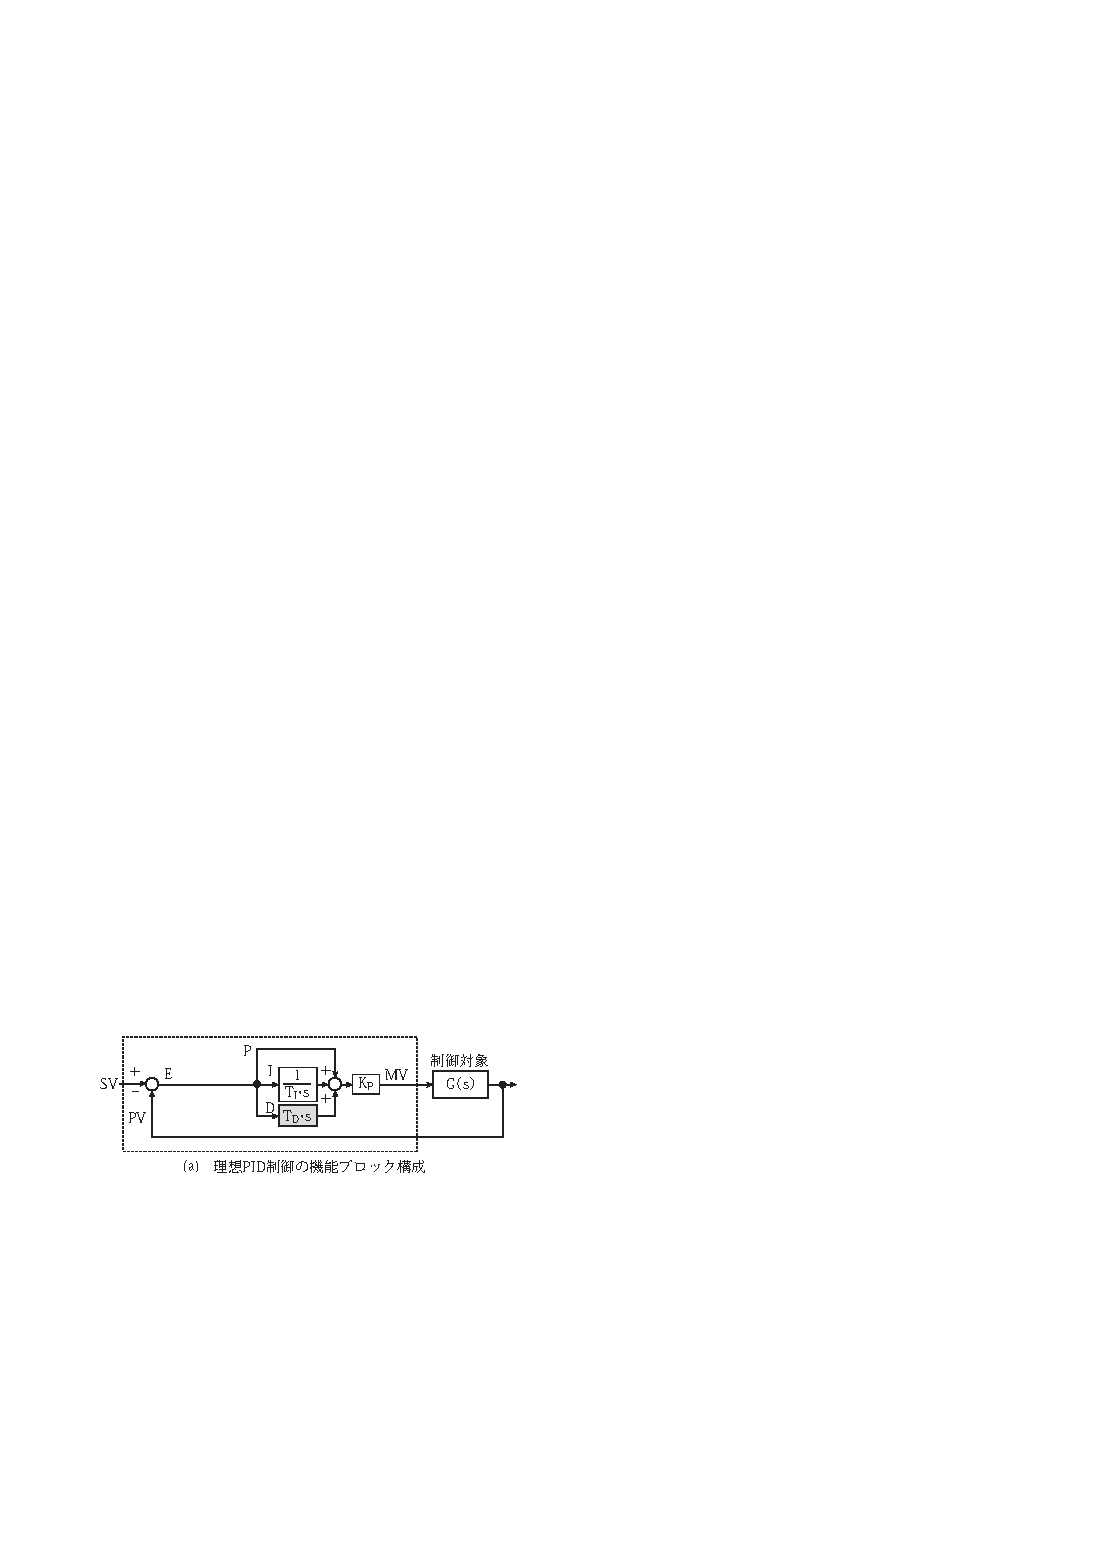
\includegraphics[width=0.8\hsize]{pid_ideal_block.pdf}
  \caption{理想PID制御のブロック図}
  \label{pid_ideal_block}
\end{figure}

\clearpage
理想PID制御の持つ、ノイズに弱いという欠点を解決するために、ノイズを抑制するローパスフィルタ(一次遅れフィルタ)を組み込んだ制御を実用PID制御という。実用PID制御のブロック図を以下の図\ref{pid_practice_block}に示す。
\begin{figure}[htbp]
  \centering
  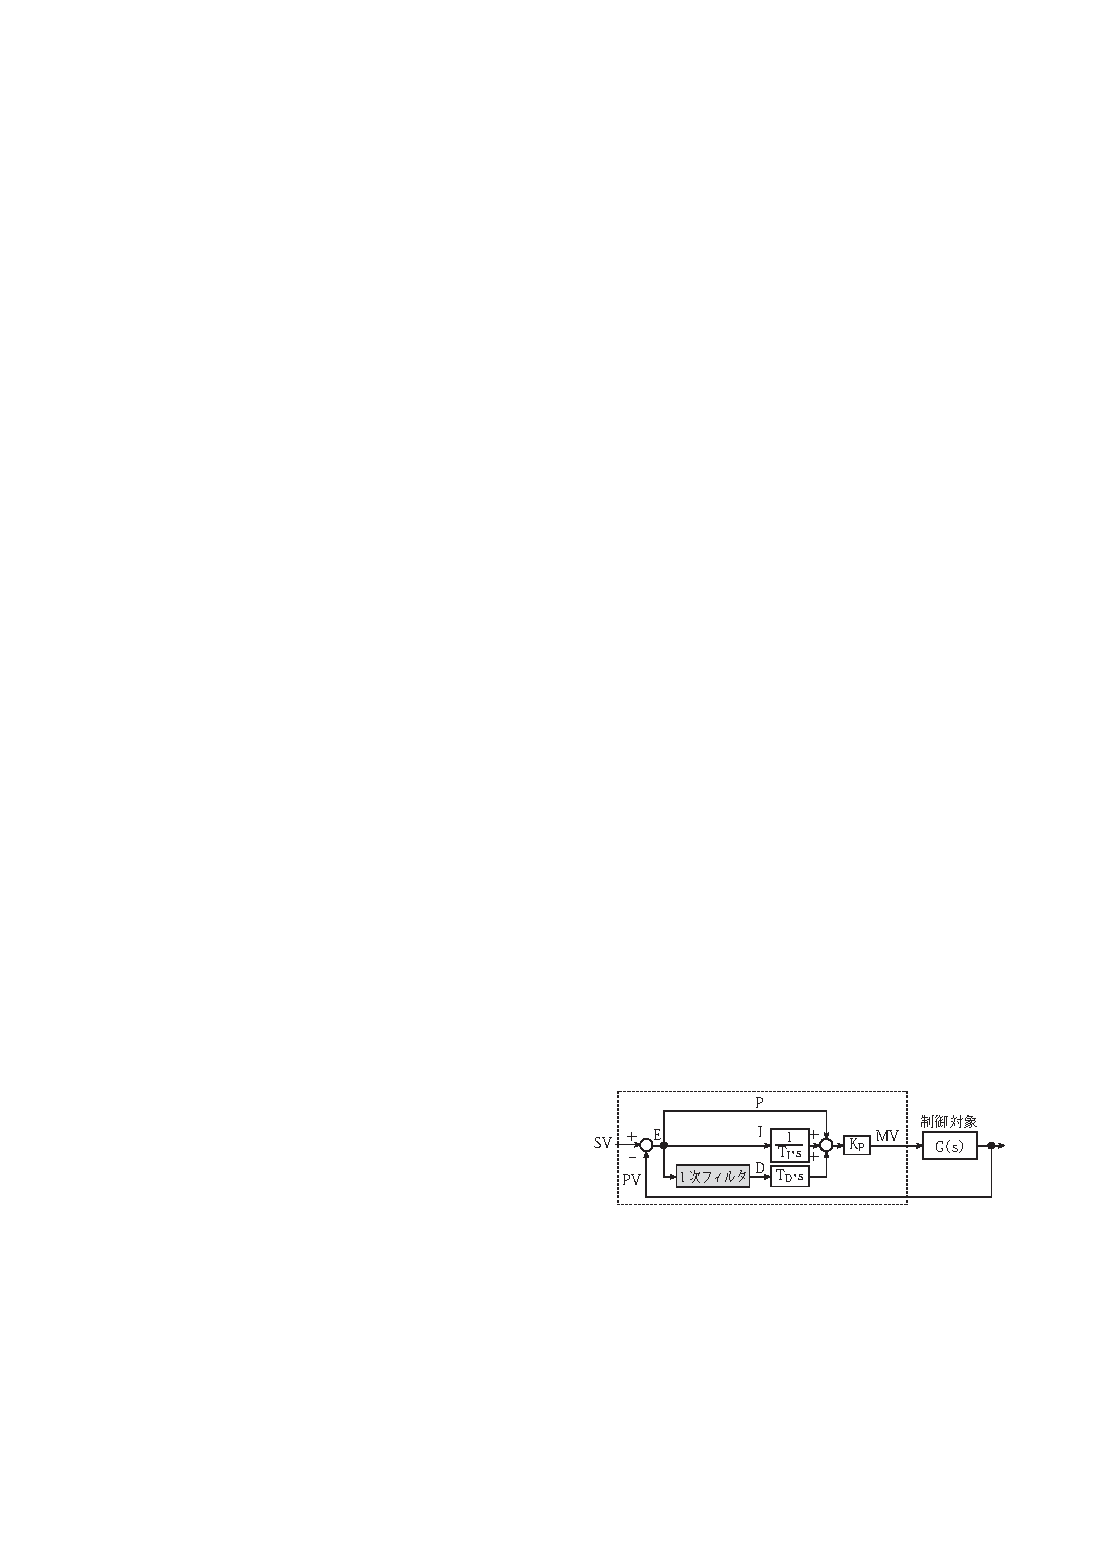
\includegraphics[width=0.8\hsize]{pid_practice_block.pdf}
  \caption{実用PID制御のブロック図}
  \label{pid_practice_block}
\end{figure}
実用PID制御を伝達関数で表現すると、以下の式(\ref{eq:PID_practice4})になり、ブロック図は図\ref{pid_practice_block2}のようになる。このように、フィルタを導入した微分制御のことを不完全微分という。ここで$\eta$は微分係数という定数であり、通常0.1から0.125の値を設定する\cite{実用PIDに向けての工夫その1}
\begin{eqnarray}
  C(t) &=& \frac{U(s)}{E(s)} = K_p \cdot \{1 + \frac{1}{T_i \cdot s}  +  \frac{T_d \cdot s}{1 + \eta \cdot T_d \cdot s}\}
  \label{eq:PID_practice4}
\end{eqnarray}
\begin{figure}[htbp]
  \centering
  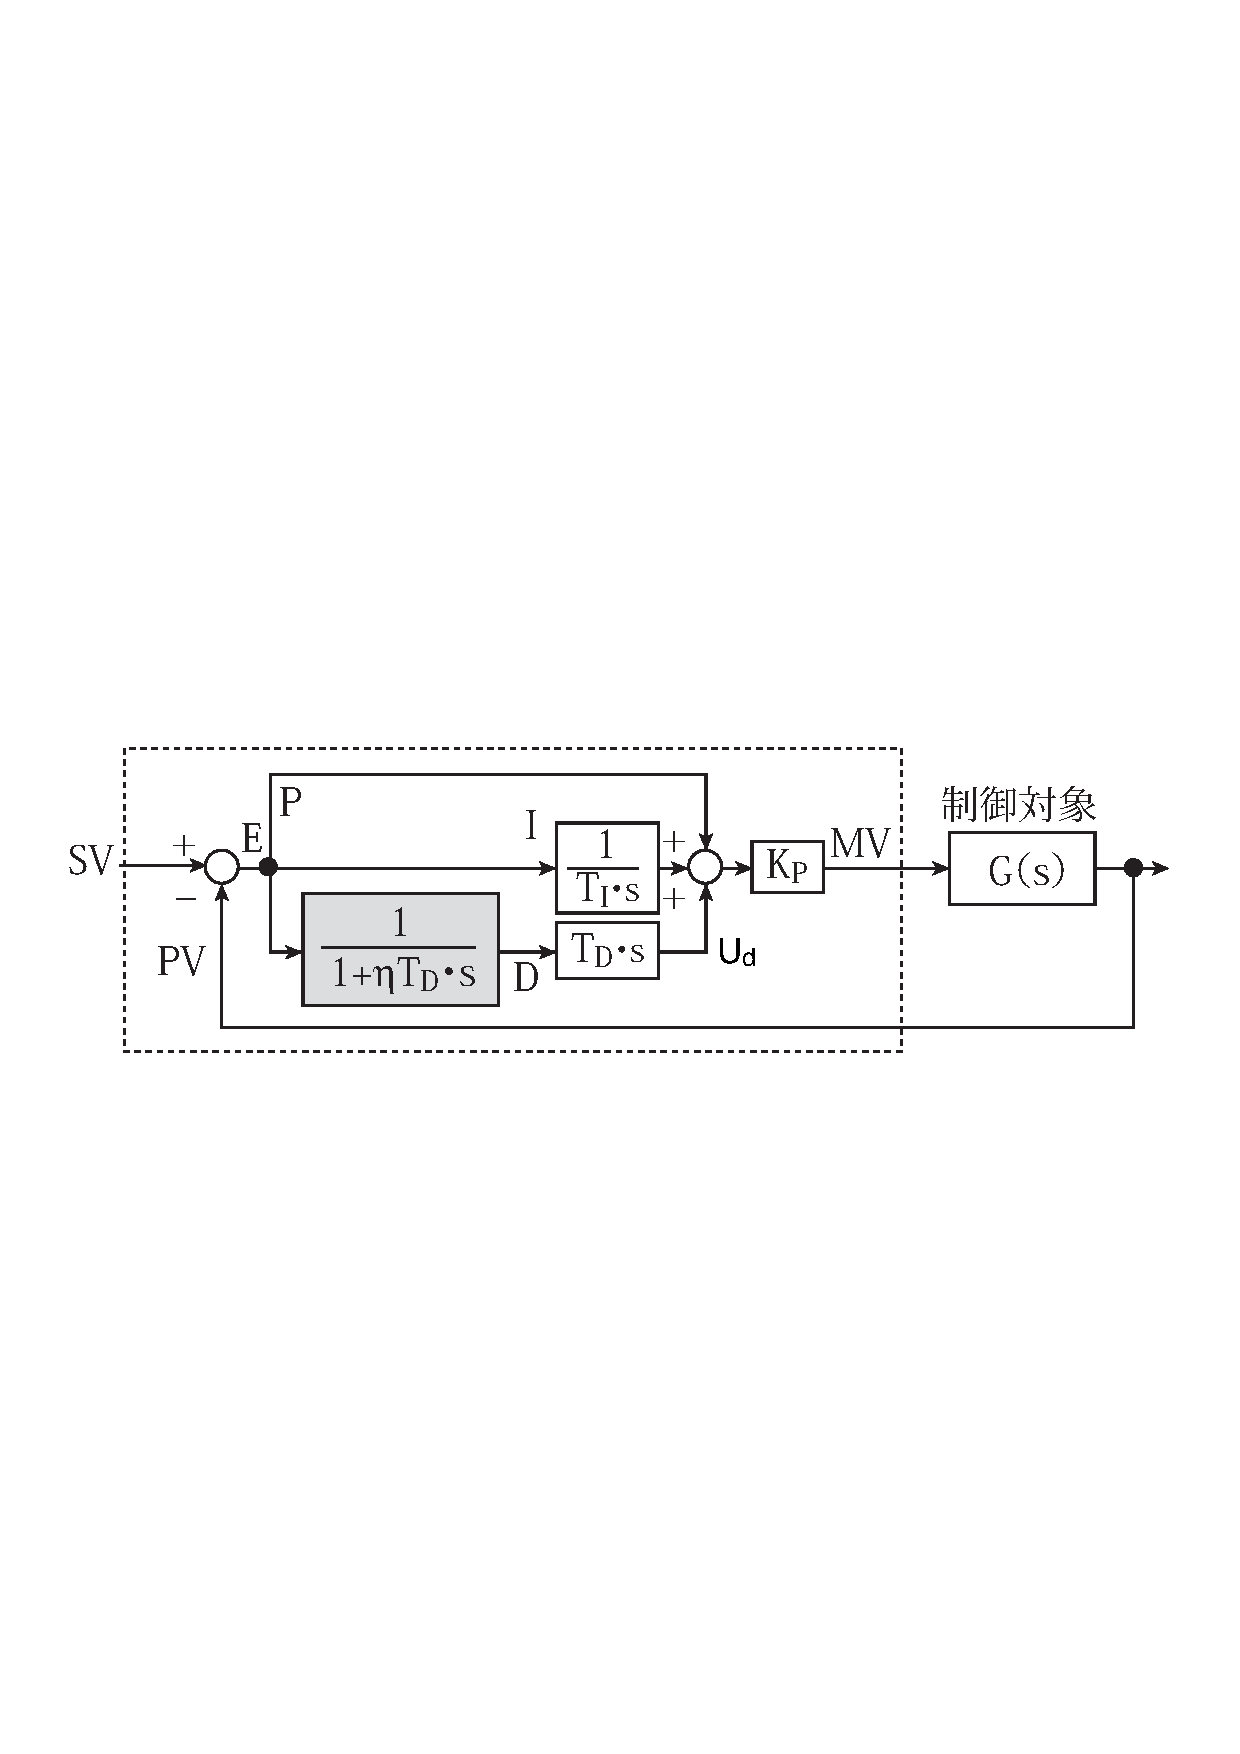
\includegraphics[width=0.8\hsize]{pid_practice_block2.pdf}
  \caption{実用PID制御のブロック図(伝達関数での表現)}
  \label{pid_practice_block2}
\end{figure}


式(\ref{eq:PID_practice4})に示した伝達関数のうち、微分制御に関する部分を抽出した式を以下の式(\ref{eq:D_practice})に示す。
\begin{eqnarray}
  U_d(s) &=& \frac{T_d \cdot s}{1 + \eta \cdot T_d \cdot s} \cdot E(s)
  \label{eq:D_practice}
\end{eqnarray}
式(\ref{eq:D_practice})を式(\ref{eq:D_practice1})のように式変形する。
\begin{eqnarray}
  U_d(s) \cdot (1 + \eta \cdot T_d \cdot s) &=& T_d \cdot s \cdot E(s)\nonumber\\
  U_d(s) + \eta \cdot T_d \cdot s \cdot U_d(s) &=& T_d \cdot s \cdot E(s)
  \label{eq:D_practice1}
\end{eqnarray}
そして、逆ラプラス変換を行うことにより、通常の微分方程式になる(\ref{eq:D_practice2})。
\begin{eqnarray}
  \mathcal{L}^{-1}[U_d(s) + \eta \cdot T_d \cdot s \cdot U_d(s)] &=& \mathcal{L}^{-1}[T_d \cdot s \cdot E(s)]\nonumber\\
  u_d(t) + \eta \cdot T_d \cdot \frac{d}{dt}u_d(t) &=& T_d \cdot \frac{d}{dt}e(t)\nonumber\\
  u_d(t) &=& T_d (\frac{d}{dt}e(t) - \eta \cdot \frac{d}{dt}u_d(t))
  \label{eq:D_practice2}
\end{eqnarray}

以上の議論より、実用PID制御は以下の式で表すことができる。
(※右辺に$u_d(t)$が残っており、微分方程式になっている。そのため、プログラムで実装する際には、後進差分近似を行った上で微分方程式を解く必要がある(補足))
\begin{eqnarray}
  u(t) &=& K_p \cdot \{e(t) + \frac{1}{T_i} \cdot \int_0^t e(\tau) d\tau +  T_d (\frac{d}{dt}e(t) - \eta \cdot \frac{d}{dt}u_d(t))\}
  \label{eq:PID_practice5}
\end{eqnarray}
\clearpage

\section{移動平均、実用PID制御}
表\ref{table:Ziegler-Nichols_setting}に示したPID制御の値を$K_p$、$K_i$および$K_d$にそれぞれ設定し、シグナリング頻度($s(t)$)を指数移動平均で平滑化した値($\overline{s(t)}$)をPID制御への入力とした場合の評価結果を図\ref{result_pid_average}に示す($\alpha = 0.125$)。
\begin{eqnarray}
  \overline{s(t)} &=& \alpha  \cdot s(t) + (1 - \alpha) \cdot \overline{s(t-1)}
  \label{eq:PID_average}
\end{eqnarray}
\begin{figure}[htbp]
  \begin{center}
    \begin{tabular}{c}
      \begin{minipage}{0.45\hsize}
        \begin{center}
        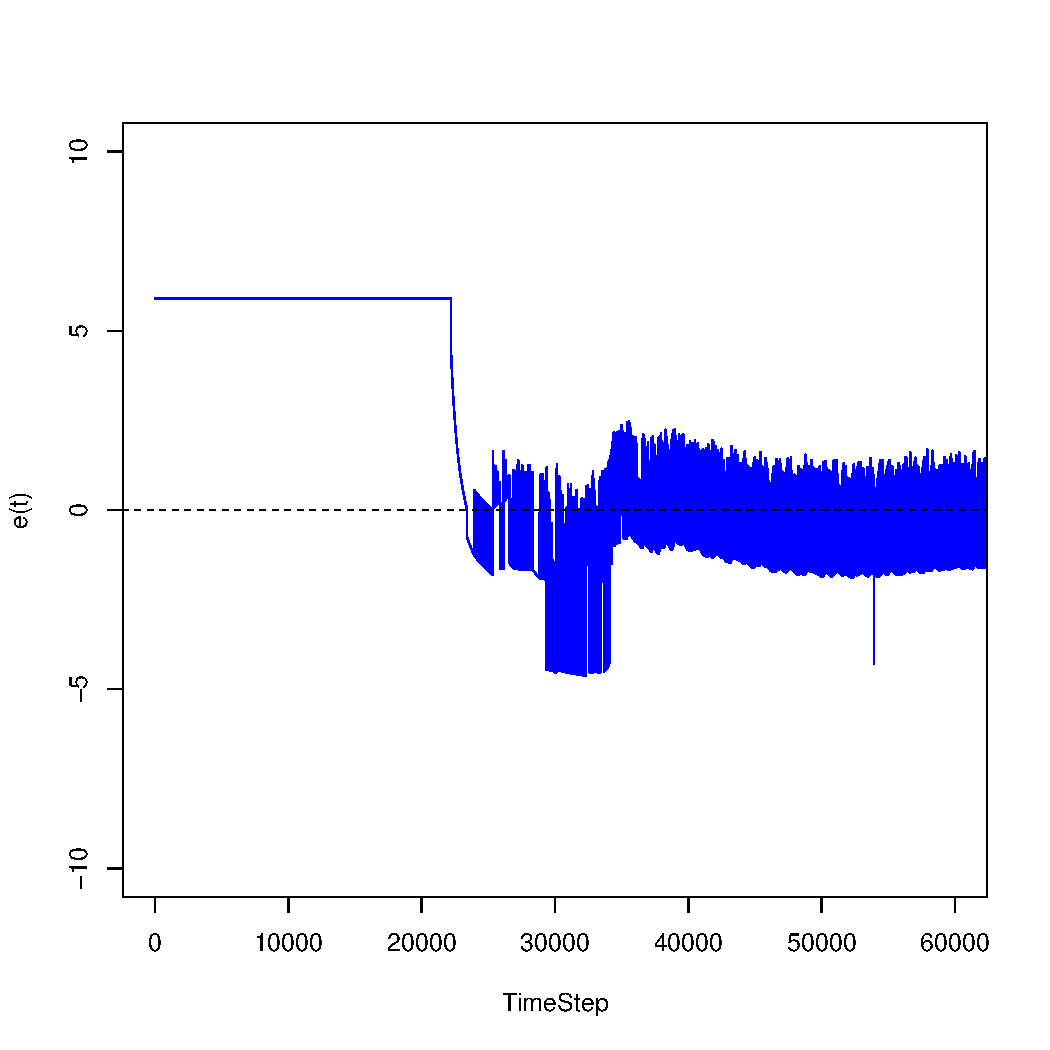
\includegraphics[width=1\hsize]{scenario_5_e_86400_345600_0-318_3725_931-25_0-125_average.pdf}
        \subcaption{$e(t)$の変化($K_p = 0.318、K_i = 0.0000854、K_d = 296.14$、指数移動平均)}
        \label{scenario_5_e_86400_345600_0-318_0-318_3725_931-25_0-125_average}
        \end{center}
      \end{minipage}
      \begin{minipage}{0.45\hsize}
        \begin{center}
        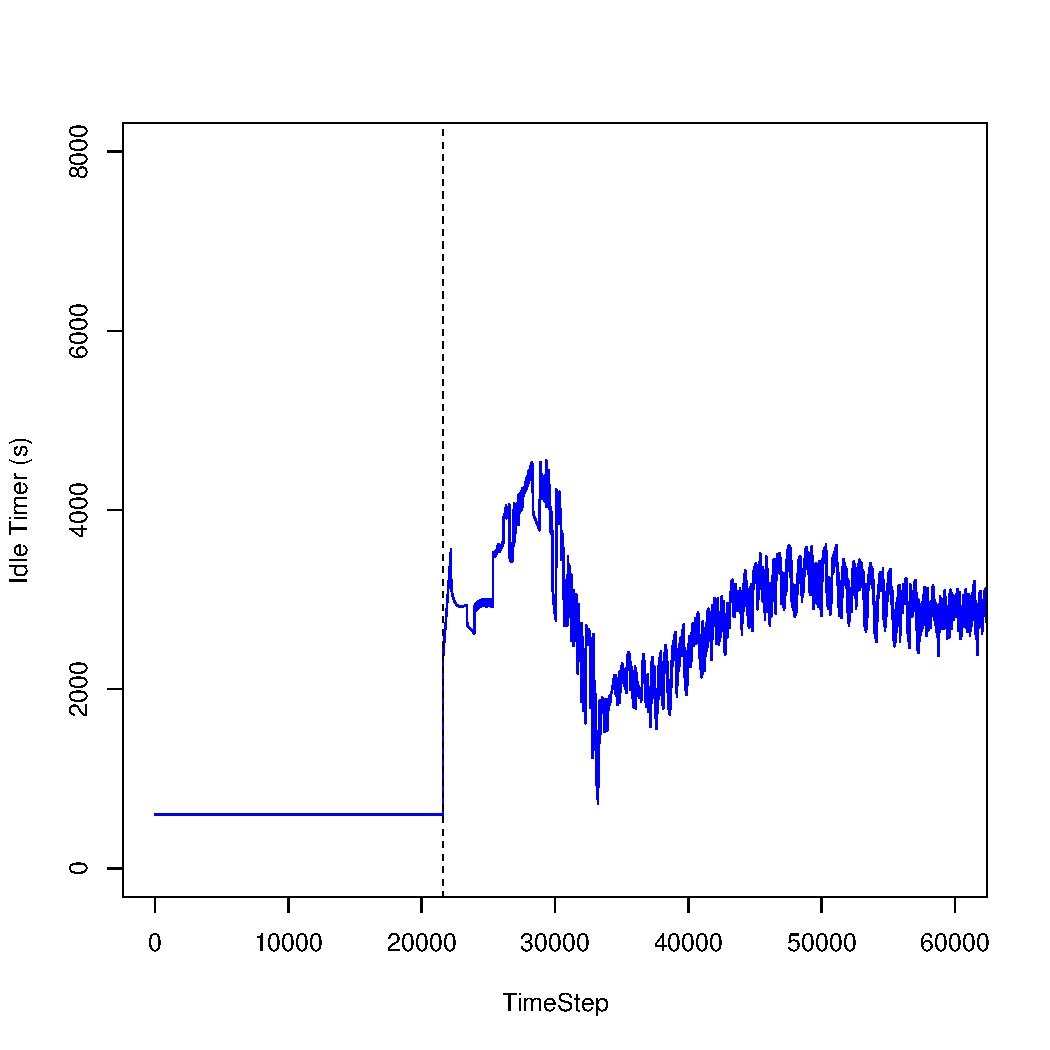
\includegraphics[width=1\hsize]{scenario_5_idleTimer_86400_345600_0-318_3725_931-25_0-125_average.pdf}
        \subcaption{IdleTimerの変化($K_p = 0.318、K_i = 0.0000854、K_d = 296.14$、指数移動平均)}
        \label{scenario_5_idleTimer_86400_345600_0-318_3725_931-25_0-125_average}
        \end{center}
      \end{minipage}\\
      \begin{minipage}{0.45\hsize}
        \begin{center}
        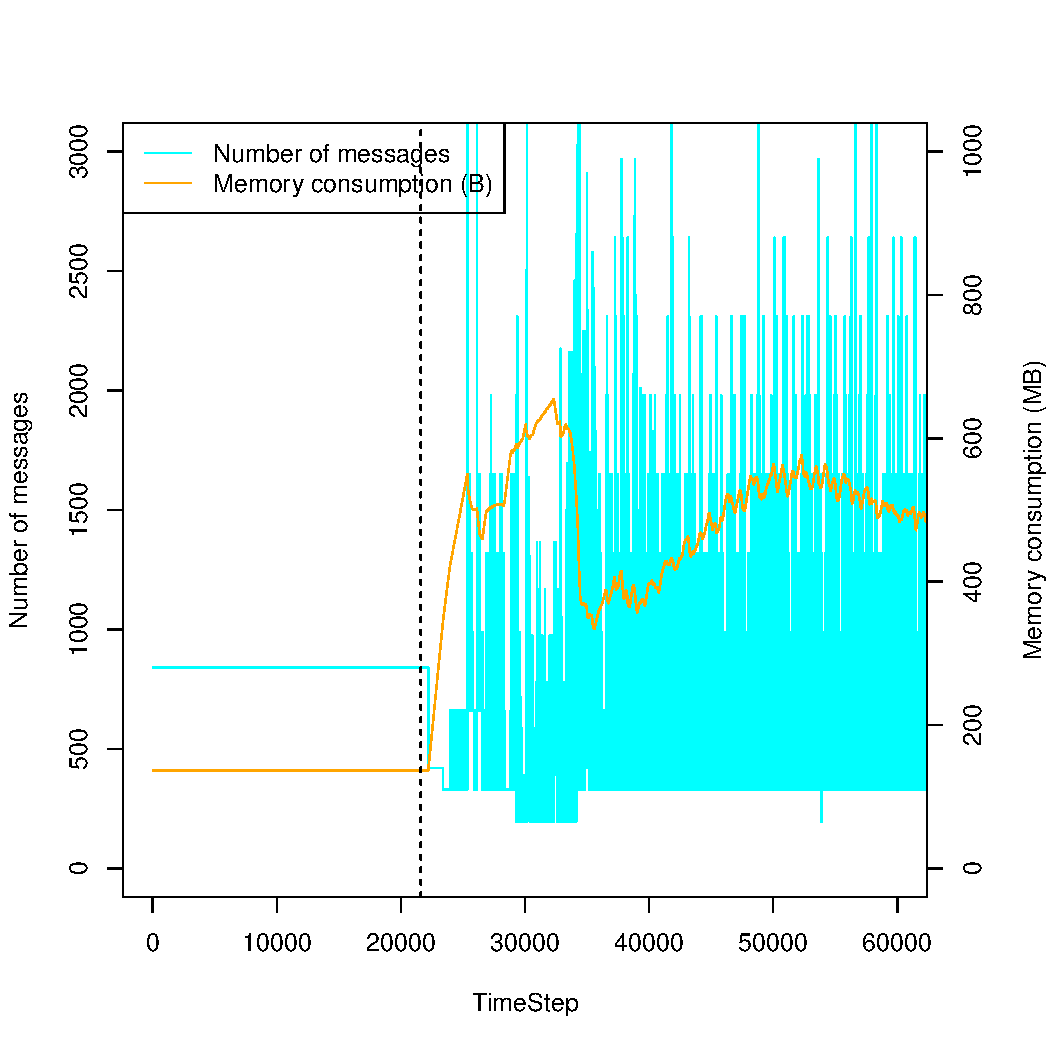
\includegraphics[width=1\hsize]{scenario_5_signaling_and_memoryload_vs_timeStep_86400_345600_0-318_3725_931-25_0-125_average.pdf}
        \subcaption{CPU負荷とメモリ使用量の変化($K_p = 0.318、K_i = 0.0000854、K_d = 296.14$、指数移動平均)}
        \label{scenario_5_signaling_and_memoryload_vs_timeStep_86400_345600_0-318_3725_931-25_0-125_average}
        \end{center}
      \end{minipage}
      \begin{minipage}{0.45\hsize}
        \begin{center}
        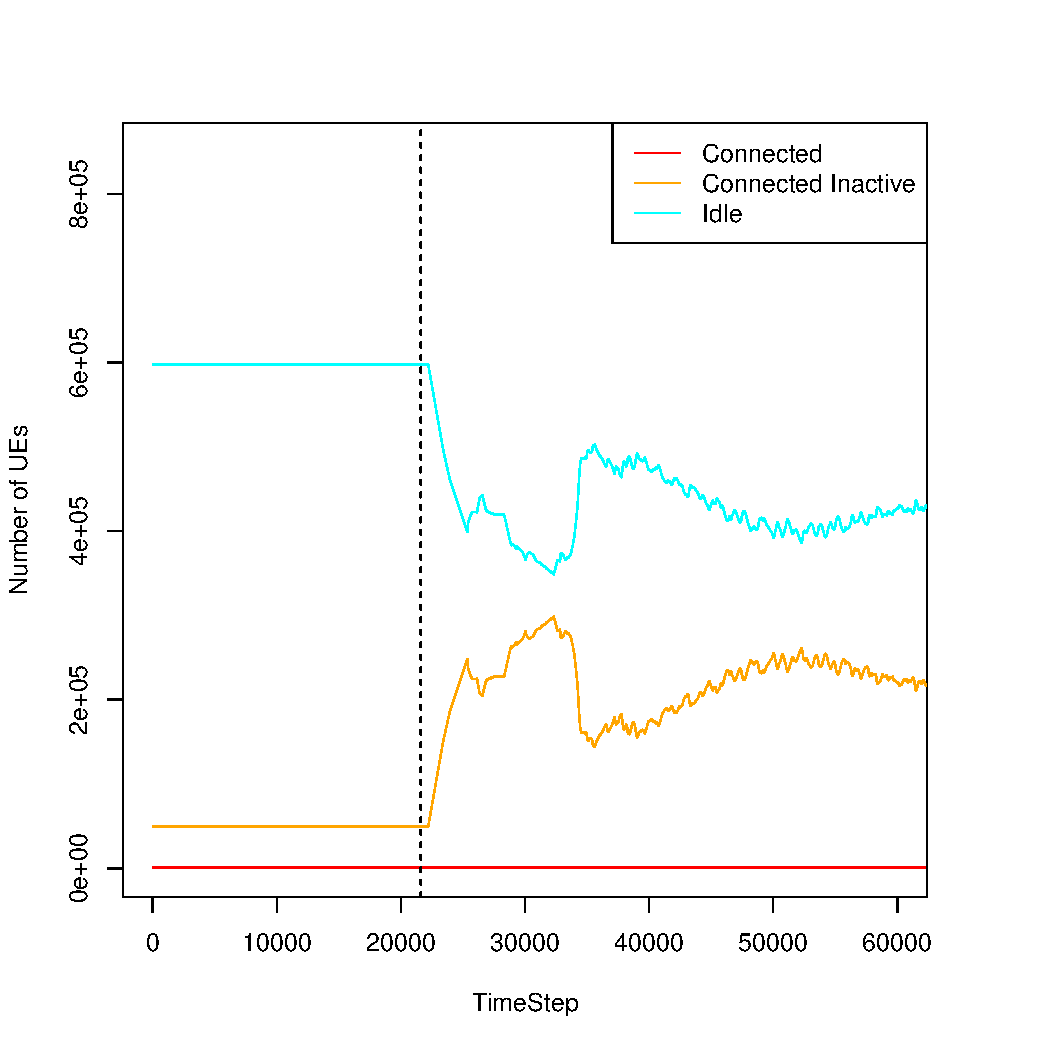
\includegraphics[width=1\hsize]{scenario_5_stateBreakdown_86400_345600_0-318_3725_931-25_0-125_average.pdf}
        \subcaption{各状態にあるUE台数の変化($K_p = 0.318、K_i = 0.0000854、K_d = 296.14$、指数移動平均)}
        \label{scenario_5_stateBreakdown_86400_345600_0-318_3725_931-25_0-125_average}
        \end{center}
      \end{minipage}
    \end{tabular}
    \caption{}
    \label{result_pid_average}
  \end{center}
\end{figure}

\clearpage
表\ref{table:Ziegler-Nichols_setting}に示したPID制御の値をPID制御の値を$K_p$、$K_i$および$K_d$にそれぞれ設定し、ローパスフィルタを用いた実用PID制御を行った場合の評価結果を図\ref{result_pid_practice}に示す。
\begin{figure}[htbp]
  \begin{center}
    \begin{tabular}{c}
      \begin{minipage}{0.45\hsize}
        \begin{center}
        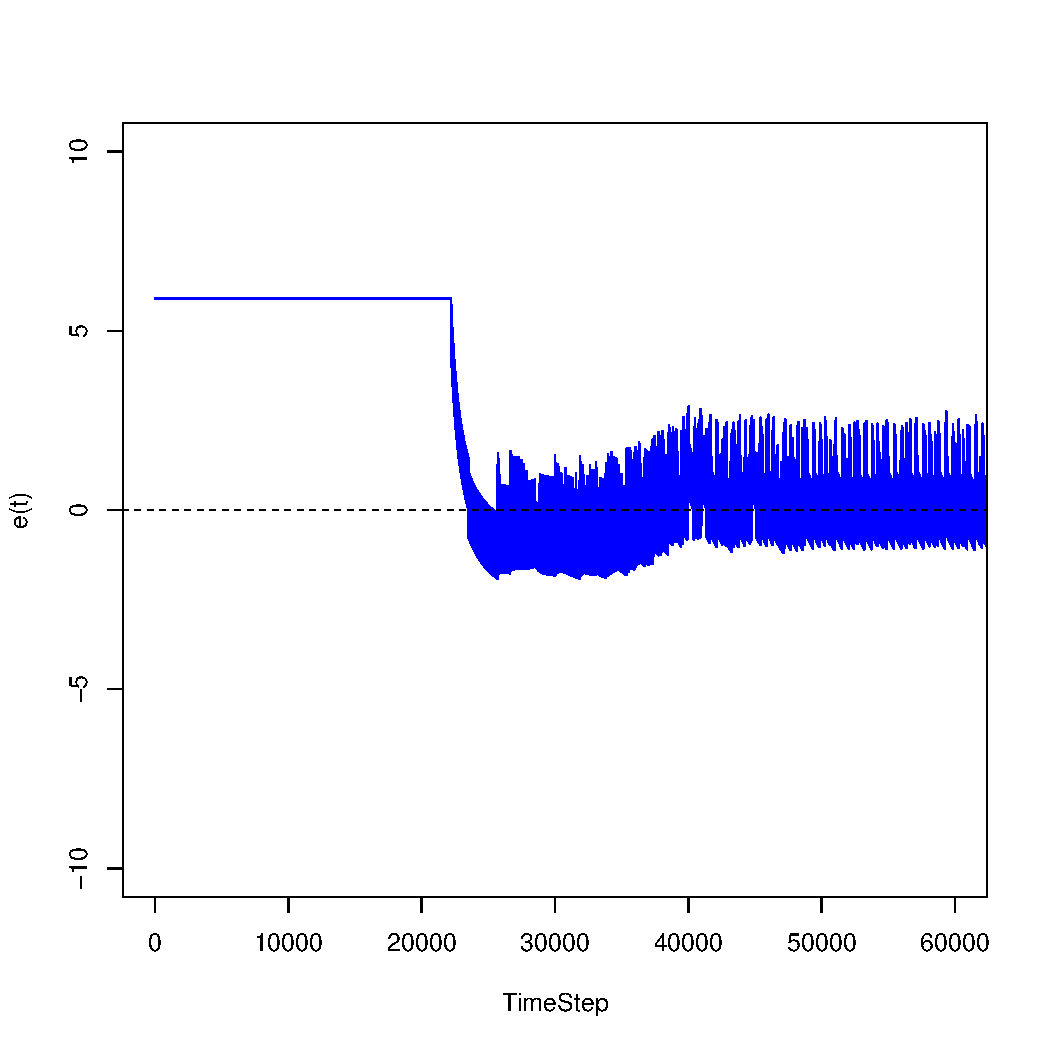
\includegraphics[width=1\hsize]{scenario_5_e_86400_345600_0-318_3725_931-25_0-125_practice.pdf}
        \subcaption{$e(t)$の変化($K_p = 0.318、K_i = 0.0000854、K_d = 296.14$、実用PID)}
        \label{scenario_5_e_86400_345600_0-318_0-318_3725_931-25_0-125_practice}
        \end{center}
      \end{minipage}
      \begin{minipage}{0.45\hsize}
        \begin{center}
        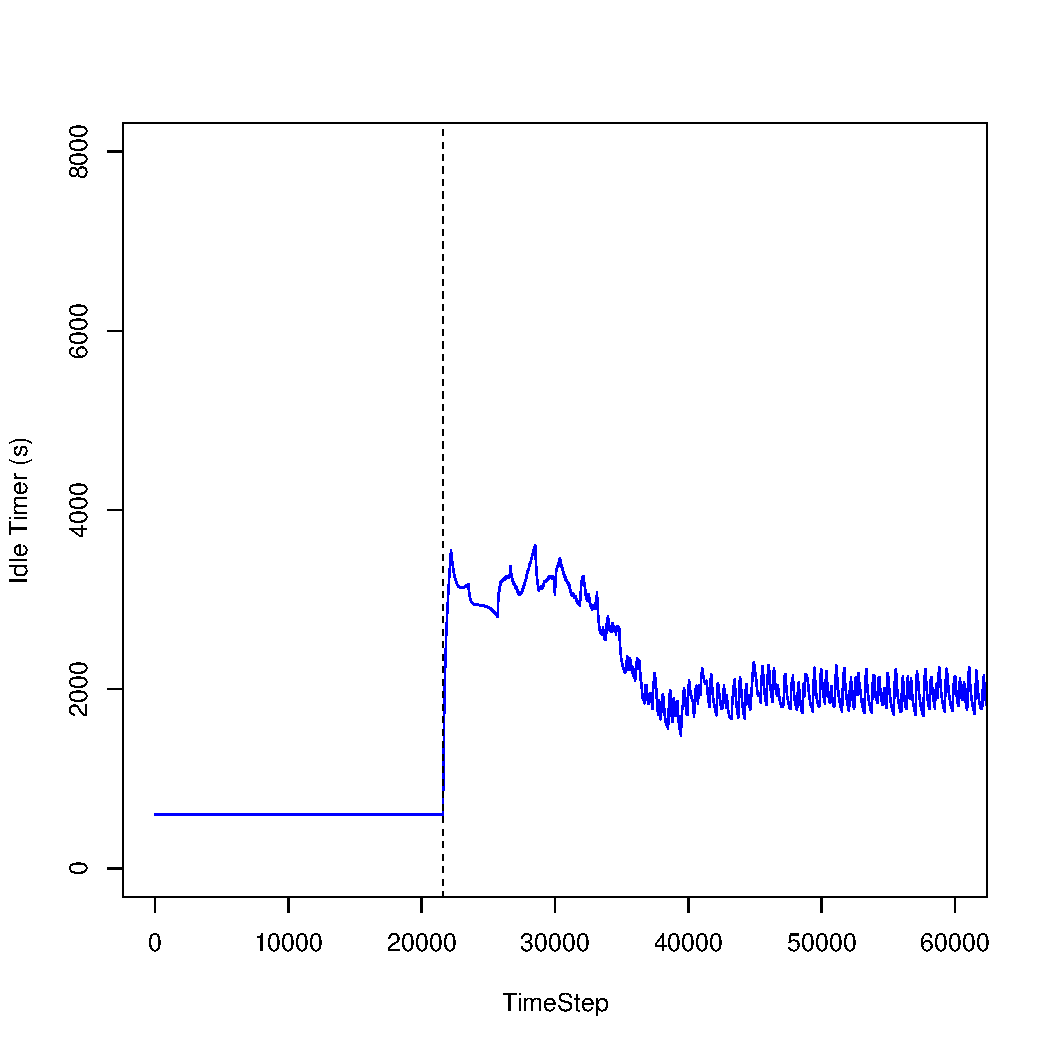
\includegraphics[width=1\hsize]{scenario_5_idleTimer_86400_345600_0-318_3725_931-25_0-125_practice.pdf}
        \subcaption{IdleTimerの変化($K_p = 0.318、K_i = 0.0000854、K_d = 296.14$、実用PID)}
        \label{scenario_5_idleTimer_86400_345600_0-318_3725_931-25_0-125_practice}
        \end{center}
      \end{minipage}\\
      \begin{minipage}{0.45\hsize}
        \begin{center}
        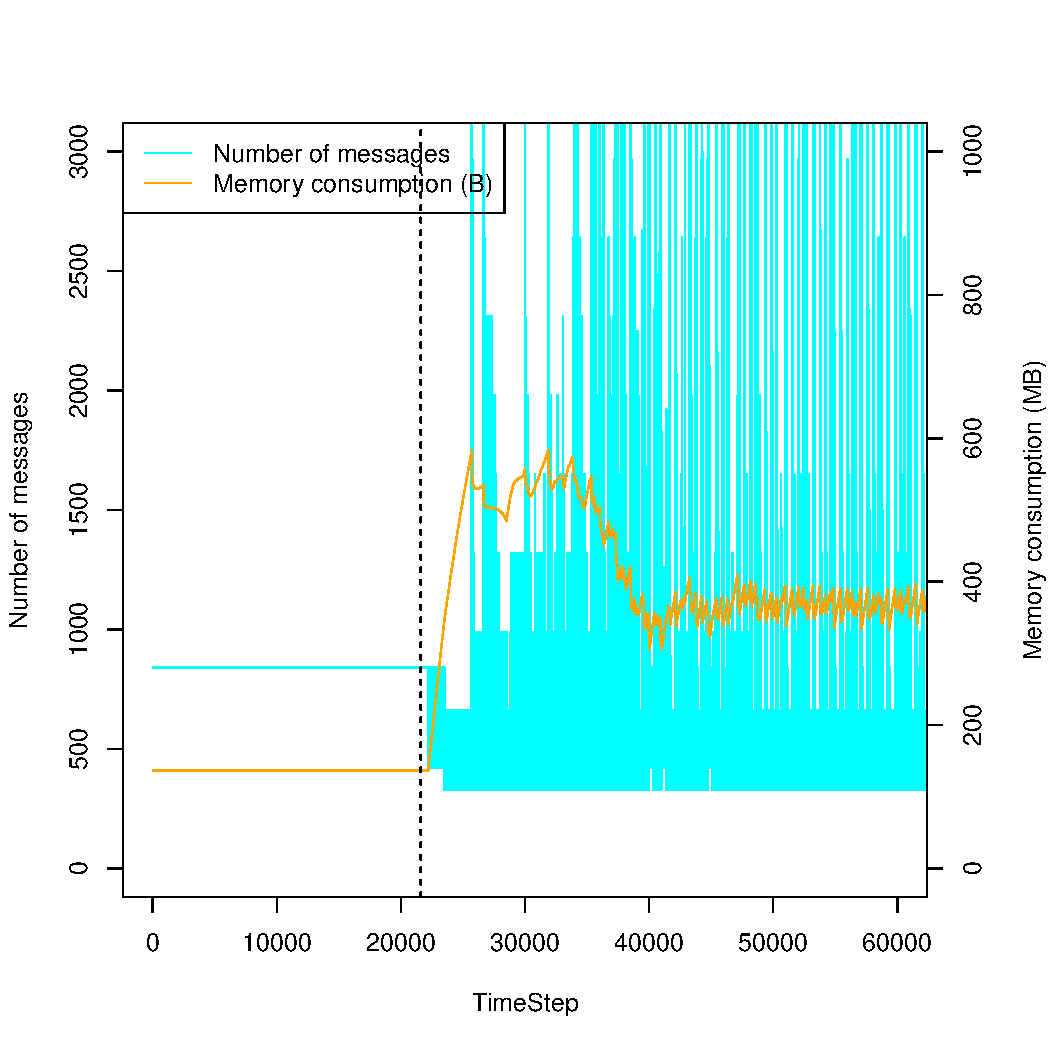
\includegraphics[width=1\hsize]{scenario_5_signaling_and_memoryload_vs_timeStep_86400_345600_0-318_3725_931-25_0-125_practice.pdf}
        \subcaption{CPU負荷とメモリ使用量の変化($K_p = 0.318、K_i = 0.0000854、K_d = 296.14$、実用PID)}
        \label{scenario_5_signaling_and_memoryload_vs_timeStep_86400_345600_0-318_3725_931-25_0-125_practice}
        \end{center}
      \end{minipage}
      \begin{minipage}{0.45\hsize}
        \begin{center}
        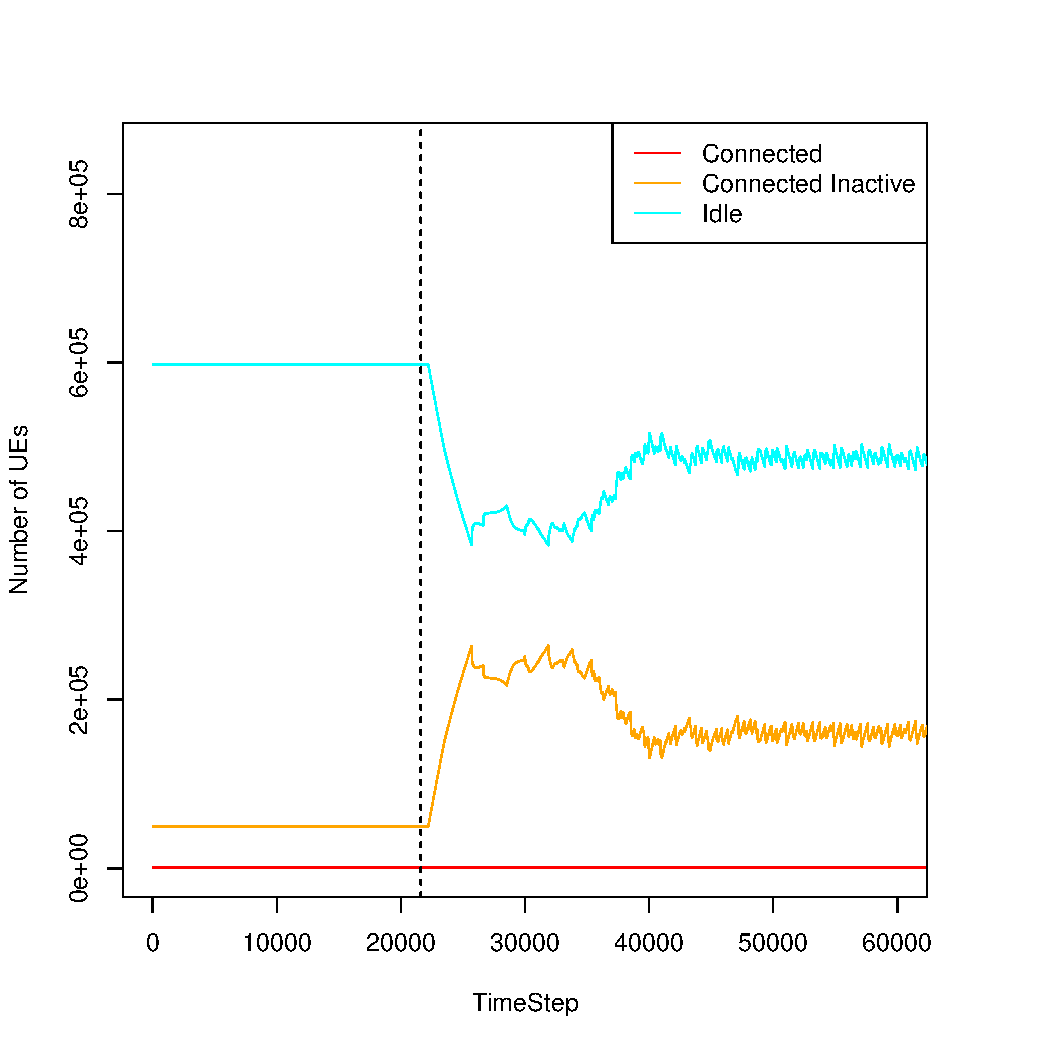
\includegraphics[width=1\hsize]{scenario_5_stateBreakdown_86400_345600_0-318_3725_931-25_0-125_practice.pdf}
        \subcaption{各状態にあるUE台数の変化($K_p = 0.318、K_i = 0.0000854、K_d = 296.14$、実用PID)}
        \label{scenario_5_stateBreakdown_86400_345600_0-318_3725_931-25_0-125_practice}
        \end{center}
      \end{minipage}
    \end{tabular}
    \caption{}
    \label{result_pid_practice}
  \end{center}
\end{figure}

\clearpage
図\ref{result_pid_average}および図\ref{result_pid_practice}の結果より、指数移動平均や実用PID制御を用いて入力の離散的な変動を平滑化することによって、そのようにしない場合(図\ref{result_pid})と比較して制御が安定することがわかる。しかし、依然としてIdleタイマの制御が十分安定しているとは言えない。指数移動平均の荷重($\alpha$)や実用PID制御における微分係数($\eta$)の値を変更しても同様に、Idleタイマが安定することはなかった。

図\ref{result_pid_average}に示したIdleタイマの変化とシグナリング頻度の変化をタイムステップ50,000から55,000の範囲でプロットしたグラフを図\ref{scenario_5_analyze_86400_345600_0-318_3725_931-25_0-125_average}に示す。この図を見ると、Idleタイマおよびシグナリング頻度は周期的に変動していることがわかる。また、それぞれの変動のタイミングおよび周期が一致していることもわかる。これは、シグナリング頻度の変化にIdleタイマを追従させるようにPID制御が機能しているためである。シグナリング頻度が周期的に変化している理由は、Idleタイマの変化によって、UEの状態遷移が集中する期間が周期的に発生するためである。図中の左側に2本の破線と2本の直線を引いた。2本の破線に囲まれた期間はシグナリング頻度が大きく、Idleタイマが約3,500~sに設定されている。一方、2本の直線に囲まれた期間はシグナリング頻度が小さく、Idleタイマは約3,100~sに設定されている。すると、破線で示した期間にデータ送信を行ったUEは、約3,500~s後にConnected Inactive 状態からアイドル状態への状態遷移を発生させる。同様に、直線で示した期間にデータ送信を行ったUEは、約3,100~s後に状態遷移を発生させる。このタイミングを図中の右側の破線および直線に示す。右側の破線および直線は左側の破線および直線のそれぞれ3,500~s、3,100~s後を示している。これを見ると、UEの状態遷移のタイミングが重なっていることがわかる。また、それが原因となり、シグナリング頻度が大きくなっている。上述のように、シグナリング頻度の変動が、一定期間後に同様のシグナリング頻度の変動を引き起こす場合がある。 
\begin{figure}[htbp]
  \centering
    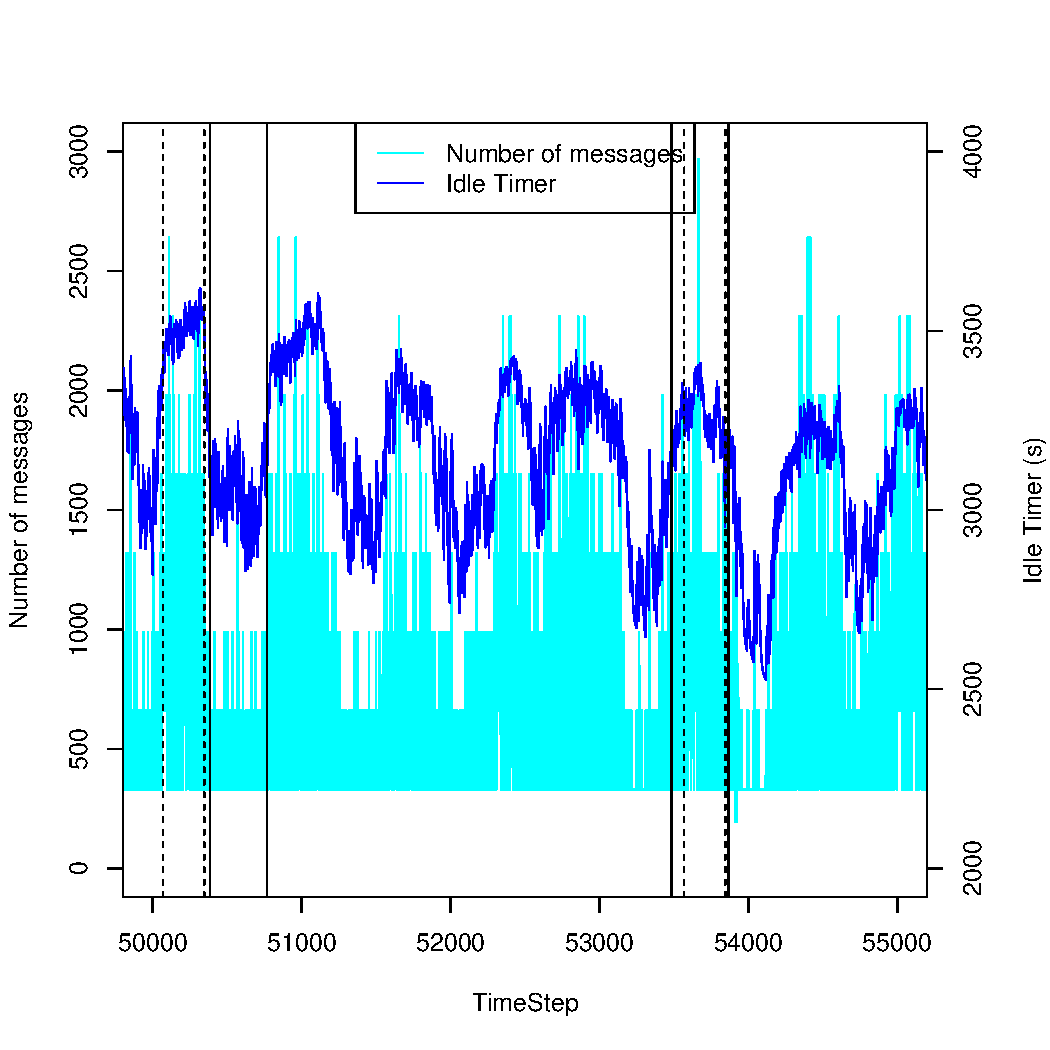
\includegraphics[width=1\hsize]{scenario_5_analyze_86400_345600_0-318_3725_931-25_0-125_average.pdf}
    \caption{IdleタイマとCPU負荷の変化($K_p = 0.318、K_i = 0.0000854、K_d = 296.14$、移動平均)}
    \label{scenario_5_analyze_86400_345600_0-318_3725_931-25_0-125_average}
\end{figure}

% 限界ゲイン$K_{pc}$=0

% 限界周期$T_c$=7450
% $K_p=0.6K_{pc}=0.318$
% $K_i=K_p / 0.5T_c = 0.318 / 3725 = 0.0000854$
% $K_d=K_p \cdot 0.125T_c = 296.14$
%T_i =
%T_d = 931.25
%29402 36863 44317 51752   7461 7454  7435

% $K_p=0.54K_{pc}=0.2862$
% $K_i=K_p / 0.83T_c = 0.2862 / 6183.5 = 0.00004628$

\section{今後の予定}
  \begin{itemize}
    \item PID制御に関する学習
    \item リソースが不足した際の制御
  \end{itemize}

\section*{\addcontentsline{toc}{section}{参考文献}}
\bibliographystyle{IEEEtran}
\bibliography{/Users/t-adachi/Documents/study/Bibliography/bib/hpt_core_network/myBib/LABbiblio,/Users/t-adachi/Documents/study/Bibliography/bib/hpt_core_network/Study_Group_Bibtex/bib/hptCoreNetwork_Study}

\section{補足}
\begin{eqnarray}
  u_d(t) &=& T_d (\frac{d}{dt}e(t) - \eta \cdot \frac{d}{dt}u_d(t))\nonumber\\
  u_d(t) &=& T_d \cdot (e(t) - e(t-1)) - \eta \cdot T_d \cdot (u_d(t) - u_d(t-1))\nonumber\\
  u_d(t) + \eta \cdot T_d \cdot u(t) &=& T_d \cdot \Delta e(t) + \eta \cdot T_d \cdot u_d(t-1)\nonumber\\
  u_d(t) &=& \frac{T_d}{1 + \eta \cdot T_d} \cdot \Delta e(t) + \frac{\eta \cdot T_d }{1 + \eta \cdot T_d}\cdot u_d(t-1)
  \label{eq:PID_practice5}\\
  \ast \Delta e(t) &=& e(t) - e(t-1)\nonumber
\end{eqnarray}
\end{document}
